\documentclass[10pt,a4paper]{article}

% ============================================================================
% Packages & Page Geometry (Overleaf Verified Order)
% ============================================================================
\usepackage[utf8]{inputenc}
\usepackage[T1]{fontenc}
\usepackage{lmodern}
\usepackage{microtype}
\usepackage[margin=0.70in]{geometry}
\usepackage{amsmath,amssymb,amsfonts,amsthm}
\usepackage{booktabs}
\usepackage{multirow}
\usepackage{array}
\usepackage{graphicx}
\usepackage{xcolor}
\usepackage{tikz}
\usepackage{pgfplots}
\usetikzlibrary{arrows.meta,positioning,shapes.geometric,calc}
\pgfplotsset{compat=1.18}
\usepackage{hyperref}

\hypersetup{
    colorlinks=true,
    linkcolor=blue!70!black,
    citecolor=blue!70!black,
    urlcolor=blue!70!black
}

\newtheorem{proposition}{Proposition}

% ============================================================================
% Title & Author Metadata (Aligned with CMPB Update Scope)
% ============================================================================
\title{\textbf{Scale-Adaptive Piecewise-Quadratic Rectifiers for Rare-Event Genomic and Multi-Domain Screening: Offset-Scale Equivalence, Mechanistic Diagnostics, and Reproducible Computational Validation}}

\author{
    \textbf{Preecha Noiumkar}$^{1,*}$ and \textbf{Thawatchai Chomsiri}$^{1}$ \\[0.4em]
    \small $^{1}$Research Center of Information Technology for the Future, Department of Information Technology, \\
    \small Faculty of Informatics, Mahasarakham University, Mahasarakham 44150, Thailand \\[0.2em]
    \small $^{*}$Corresponding author. Emails: \texttt{preecha.n@msu.ac.th} (P. Noiumkar), \texttt{thawatchai.c@msu.ac.th} (T. Chomsiri)
}
\date{}

\begin{document}
\maketitle

% ============================================================================
% Abstract
% ============================================================================
\begin{abstract}
\noindent
\textbf{Background and Objective:} Convolutional neural networks (CNNs) deployed for rare-event biomedical screening---such as candidate variant classification in high-throughput sequencing and anomaly detection---must learn minority representations under severe class imbalance ($10:1$ to $200:1$), where a degenerate classifier predicting only the majority class achieves near-perfect accuracy ($99.00\%$--$99.50\%$). Piecewise-quadratic $C^1$-continuous rectifiers such as Smooth ReLU (SmeLU, centered symmetrically on $[-\beta, +\beta]$) replace ReLU's non-differentiable kink with a parabolic transition. Recently proposed Smooth RectLU and its trainable variant AS-RectLU anchor this transition asymmetrically on $[L, L+W]$ with default $L=0, W=2$. We investigate the mechanistic causes of silent majority-class collapse in this rectifier family and develop scale-adaptive remedies validated across genomic, visual, and tabular domains. \\
\textbf{Methods:} We prove that $C^1$ smoothness itself does not cause collapse, as smooth baselines ($C^1$ ELU/SELU and $C^\infty$ GELU/SiLU/Mish/Softplus) converge reliably. Algebraically, Smooth RectLU satisfies the exact identity $f_S(x; L, W) = \text{SmeLU}_{\beta=W/2}(x - L - W/2)$, meaning that initializing at $L=0, W=2$ imposes an implicit negative bias offset ($\Delta b = -1$), a vanishing origin slope ($f'(0^+)=0$), and severe forward second-moment attenuation ($\mathbb{E}[f^2]/\mathbb{E}[x^2] = 0.0874$ vs.\ $\ge 0.3550$ for functional baselines). We derive Gaussian variance propagation recurrences ($\sigma_{l+1}^2 = \frac{3}{4W^2}\sigma_l^4$), establish backward Jacobian properties for per-sample root-mean-square scale adaptation (Symmetric $\sigma$-AS-RectLU), and execute pre-specified experiments (E1--E12) across 1D/2D sparse motif generators, step-imbalanced MNIST ($100:1$), imbalanced tabular classification ($200:1$), and stratified NIST GIAB (GRCh38 v4.2.1) benchmarks including 2D hard-negative stress tests, five handcrafted/classical ML baselines, statistical pileup callers, and DeepVariant/Clair3-style neural backbones. \\
\textbf{Results:} On low-amplitude 2D motifs ($\sigma_x = 0.22$), a synergistic Offset $\times$ Scale interaction ($\text{DiD AUROC} = +0.3633 \pm 0.1248, p = 0.0020$) causes Smooth RectLU to stagnate at 20 epochs ($\text{Median MCC} = 0.0000$) even at Adam $\epsilon = 10^{-12}$, and induces bimodal seed trapping over 50--100 epochs. While global weight scaling ($s > 1$) triggers linear-tail gradient explosion ($\|\nabla \mathcal{L}_{\text{min}}\|_2 > 8000$), output-prior logit initialization ($b_{\text{out}} = \ln(p_+/p_-)$) exacerbates early gradient starvation ($\text{MCC} = 0.6303$), and objective-level re-weighting (Weighted BCE, Focal loss) fails once dense units die ($\text{MCC} \le 0.0412$), all-layer bias compensation ($b_0 = +1.0$) restores parity with SmeLU ($\text{MCC}(\tau^*) = 0.9754$). Embedding parameter-free per-sample RMS adaptation in Symmetric $\sigma$-AS-RectLU ($\kappa \in [0.4, 2.0]$) further improves 2D hard-negative GIAB screening to $\text{MCC}(\tau^*) = 0.9846$--$0.9877$ ($\text{ECE} = 0.0036$, outperforming handcrafted mismatch/VAF heuristics at $0.3354$--$0.6143$, statistical LLR/Bayesian callers at $0.6133$--$0.6143$, and SmeLU at $0.9754$), eliminates catastrophic collapse in Clair3-style ($\text{MCC}: 0.0000 \to 0.9722$) and DeepVariant-style Inception backbones ($\text{MCC}: 0.4478 \to 0.9815$), reduces training overhead by $33\%$ relative to differentiable RMS and LayerNorm via stop-gradient scale locking, preserves detection across $50\times \to 10\times$ read-depth downsampling, and achieves top performance on unit-$L_2$-normalized 1D $k$-mers ($\text{AUROC} = 0.9797 \pm 0.0022$) and $200:1$ Tabular data ($\text{MCC} = 0.4581 \pm 0.0355$). \\
\textbf{Conclusions:} Majority-class stagnation in asymmetric piecewise-quadratic rectifiers stems from negative initialization offset interacting with scale-width mismatch and imbalance-driven drift. Symmetric $\sigma$-AS-RectLU and hybrid dense architectures provide computationally efficient, calibration-stable remedies for rare-event screening.

\vspace{0.4em}
\noindent\textbf{Keywords:} Activation function; Piecewise-quadratic rectifier; Smooth RectLU; SmeLU; Scale adaptation; Class imbalance; Genomic variant screening; Genome in a Bottle
\end{abstract}

% ============================================================================
% 1. Introduction
% ============================================================================
\section{Introduction}
Convolutional neural networks (CNNs) underpin modern germline variant screening and candidate classification pipelines in high-throughput sequencing~\cite{poplin2018,luo2019,eraslan2019} as well as visual and tabular anomaly detectors~\cite{johnson2019,buda2018}. The Genome in a Bottle (GIAB) consortium provides benchmark genotype calls~\cite{zook2014,zook2019} and standardized stratification protocols~\cite{krusche2019,olson2022} for evaluating genomic classifiers. In window-level candidate screening, minority positive events typically constitute $0.5\%$ to $9.1\%$ of examples ($10:1$ to $200:1$ imbalance). In such regimes, overall accuracy is dominated by majority negatives, requiring evaluation via the Matthews correlation coefficient (MCC)~\cite{chicco2020,boughorbel2017}, area under the precision-recall curve (AUPRC)~\cite{saito2015,davis2006}, area under the ROC curve (AUROC), expected calibration error (ECE), and explicit confusion counts~\cite{branco2016}. Because severe prior imbalance shifts raw output logits negatively ($\ln(p_+/p_-) \approx -2.3$ to $-5.3$), evaluation must rigorously distinguish between \textit{threshold miscalibration} (where ranking AUROC is high and selecting an order-statistic threshold $\tau^*$ on validation data restores MCC) and \textit{optimization stagnation / majority-class collapse} (where multi-layer variance contraction stalls parameter updates, leaving AUROC near chance or trapping random seeds permanently).

Piecewise-quadratic $C^1$ rectifiers replace the non-differentiable kink of ReLU~\cite{nair2010,glorot2011} with a parabolic transition using elementary arithmetic operations. Shamir et al.~\cite{shamir2020} introduced Smooth ReLU (SmeLU) by centering a quadratic transition symmetrically over $[-\beta, +\beta]$ (threshold $L = -\beta$, width $W = 2\beta$). More recently, Chomsiri and Noiumkar~\cite{chomsiri2026} proposed RectLU and its $C^1$ variant Smooth RectLU, anchoring the transition over $[L, L+W]$ with an asymmetric default of $L=0, W=2$, alongside an adaptive variant (AS-RectLU) where $L$ and $W$ are trained via backpropagation~\cite{he2015,apicella2019,dubey2022}.

When deploying Smooth RectLU ($L=0, W=2$) and AS-RectLU on imbalanced genomic and spatial benchmarks, we observed silent majority-class collapse: models achieved accuracy equal to the majority-class rate ($98.00\%$--$99.44\%$) while predicting zero positives ($\text{MCC}(0.50) = 0.0000$). An intuitive hypothesis is that $C^1$ smoothness itself starves weak minority-class gradients. However, our evaluation across twelve activation baselines directly refutes this interpretation: $C^1$-smooth activations (ELU~\cite{clevert2016}, SELU~\cite{klambauer2017}) and $C^\infty$-smooth activations (GELU~\cite{hendrycks2016}, SiLU~\cite{ramachandran2017}, Mish~\cite{misra2020}, Softplus) train normally without collapse.

Instead, a fundamental algebraic identity governs this entire family: for any threshold $L \in \mathbb{R}$ and transition width $W > 0$, Smooth RectLU is an exact shifted copy of symmetric SmeLU:
\begin{equation}
    f_S(x; L, W) = \text{SmeLU}_{\beta = W/2}\!\left(x - L - \frac{W}{2}\right).
    \label{eq:smelu_identity}
\end{equation}
In any layer with a learnable bias vector $\mathbf{b}$, applying $f_S(\mathbf{W}\mathbf{h} + \mathbf{b}; L, W)$ is representationally identical to applying symmetric $\text{SmeLU}_{\beta=W/2}(\mathbf{W}\mathbf{h} + \mathbf{b}_{\text{eff}})$ with shifted effective bias $\mathbf{b}_{\text{eff}} = \mathbf{b} - (L + W/2)\mathbf{1}$. Despite having identical representational capacity, multi-layer networks initialized with $L=0$ and wide $W$ relative to input scale $\sigma_x$ suffer from a synergistic interaction ($\text{H1} \times \text{H2}$) when trained on imbalanced data:
\begin{itemize}
    \item \textbf{Factor H1 (Scale-Width Mismatch $\sigma_l \ll W$, Loss of Positive Homogeneity, and Second-Moment Contraction):} Unlike ReLU ($f(\alpha x) = \alpha f(x)$), any fixed-width piecewise-quadratic rectifier breaks scale invariance. When pre-activations have small amplitude relative to transition width ($\sigma_l / W \ll 1$), signals fall inside the quadratic ramp where forward variance contracts super-linearly ($\sigma_{l+1}^2 \propto (\sigma_l / W)^2 \sigma_l^2$)~\cite{poole2016,schoenholz2017,hayou2019}. At $L=0, W=2$, Smooth RectLU transmits a forward second-moment gain of only $\mathbb{E}[f^2]/\mathbb{E}[x^2] = 0.0874$ compared to $\ge 0.3550$ for all functional baselines.
    \item \textbf{Factor H2 (Implicit Negative Bias Offset $\Delta b = -(L+W/2)$, Zero Origin Slope, and Imbalance-Driven Negative Drift):} Setting $L=0$ imposes an initial negative bias offset of $\Delta b = -W/2$ relative to symmetric SmeLU and places $x=0$ at the zero-derivative boundary ($f'(0^+) = 0$). Under severe class imbalance ($99:1$ to $200:1$), overwhelming majority-class negative updates sweep pre-activations below $L=0$, triggering a dense-layer dead-unit cascade. Crucially, neither H1 nor H2 alone is sufficient to induce 2D collapse: symmetric SmeLU ($\Delta b = 0, f'(0)=0.5$) converges when $\sigma_x = 0.22$, and Smooth RectLU ($L=0, \Delta b = -1$) converges at $50:50$ class balance or when $\sigma_x = 1.00$.
\end{itemize}

The primary contributions of this study are:
\begin{enumerate}
    \item \textbf{Theoretical Dissection of Offset Equivalence, Second-Moment Recurrences, and Stop-Gradient RMSNorm Equivalence:} We establish Eq.~\eqref{eq:smelu_identity}, quantify exact Monte-Carlo moments across 19 activation configurations including shifted ($D^0$) and continuous ($C^0$) RectLU (Table~\ref{tab:moments}), formulate four quantitative predictions (Proposition~\ref{prop:h1}, P1--P4), and derive both the forward equivalence and backward Jacobian distinction between Symmetric Per-Sample $\sigma$-AS-RectLU and affine-free RMSNorm + SmeLU (Section~\ref{sec:theory}).
    \item \textbf{Mechanistic Disentanglement of Offset $\times$ Scale Interaction, All-Layer Bias Compensation, Weight Scaling Explosion, and Loss Re-Weighting:} Across controlled $2 \times 2$ factorial experiments ($\text{DiD AUROC} = +0.3633, p = 0.0020$), Adam $\epsilon = 10^{-12}$ checks, 50/100-epoch diagnostics, and initialization confound ablations (Groups A--F), we prove that compensating all hidden biases ($b_0 = +1.0$) restores exact parity with SmeLU, whereas global weight scaling ($s > 1$) triggers linear-tail gradient explosion ($\|\nabla \mathcal{L}_{\text{min}}\|_2 > 8000$), output-prior bias initialization ($b_{\text{out}} = \ln(p_+/p_-)$) worsens early gradient starvation, and objective re-weighting (Weighted BCE, Focal loss~\cite{lin2017}) cannot revive dead dense layers (Tables~\ref{tab:pathA}--\ref{tab:lw_grid} and~\ref{tab:rebuttal_suite}).
    \item \textbf{Multi-Domain, Shortcut-Controlled, and Variant-Caller Backbone Validation:} Beyond step-imbalanced MNIST ($100:1$) and Tabular ($200:1$, Table~\ref{tab:cross_domain}), we evaluate real NIST GIAB benchmarks under strict methodological controls (Tables~\ref{tab:real_giab_stratified}--\ref{tab:pipeline_hardware}): (a) per-sample unit-$L_2$-normalized 1D $k$-mers eliminating read-coverage shortcuts, (b) 2D BAM pileups stratified by variant type (SNV vs.\ Indel), zygosity (Het $0/1$ vs.\ Hom $1/1$), and read-depth downsampling ($50\times \to 10\times$), (c) a 2D hard-negative stress benchmark compared against five handcrafted/classical ML baselines, two statistical variant callers, and Clair3/DeepVariant-style neural backbones, and (d) external cohort validation on GIAB HG006--HG007.
\end{enumerate}

% ============================================================================
% 2. Related Work
% ============================================================================
\section{Related Work}
\subsection{Piecewise-Quadratic, Smooth, and Trainable Rectifiers}
ReLU~\cite{nair2010,glorot2011} resolved vanishing positive gradients at the cost of the ``dying ReLU'' phenomenon~\cite{lu2020}. Leaky ReLU~\cite{maas2013}, PReLU~\cite{he2015}, ELU~\cite{clevert2016}, SELU~\cite{klambauer2017}, GELU~\cite{hendrycks2016}, SiLU~\cite{ramachandran2017}, and Mish~\cite{misra2020} modify the negative or near-zero regime; Dubey et al.~\cite{dubey2022} provide a comprehensive survey. To achieve $C^1$ continuity without transcendental operations, Shamir et al.~\cite{shamir2020} introduced symmetric SmeLU on $[-\beta, +\beta]$, while Chomsiri and Noiumkar~\cite{chomsiri2026} proposed RectLU and $C^1$ Smooth RectLU on $[L, L+W]$ with default $L=0, W=2$. Trainable activation schemes~\cite{he2015,apicella2019} attempt to learn shape parameters via backpropagation, but suffer parameter freeze when initialized inside zero-derivative basins.

\subsection{Signal Propagation, Normalization, and Imbalanced Biomedical Classification}
Glorot and Bengio~\cite{glorot2010} and He et al.~\cite{he2015} derived variance-preserving weight initializations for linear and ReLU networks, while Mishkin and Matas~\cite{mishkin2016} (LSUV) and Scabini et al.~\cite{scabini2024} established data-driven initialization schemes. Mean-field theory~\cite{poole2016,schoenholz2017,hayou2019} characterizes how pre-activation variance $\sigma_l^2$ evolves with depth. Batch Normalization (BN)~\cite{ioffe2015}, Layer Normalization (LN), and RMS Normalization standardize pre-activation scales externally. Under severe class imbalance~\cite{johnson2019,buda2018}, cost-sensitive and focal objectives~\cite{lin2017,zhang2019} re-weight minority errors against gradient starvation~\cite{pezeshki2021}. Rigorous biomedical evaluation requires MCC~\cite{chicco2020,boughorbel2017}, AUPRC~\cite{saito2015,davis2006}, calibration metrics (ECE, Brier score), confusion counts~\cite{branco2016}, and non-parametric statistical testing with Holm-Bonferroni correction~\cite{demsar2006}.

% ============================================================================
% 3. Theoretical Analysis and Scale-Adaptive Formulations
% ============================================================================
\section{Theoretical Analysis and Scale-Adaptive Formulations}
\label{sec:theory}

\subsection{Algebraic Equivalence to Bias-Shifted SmeLU and RectLU Continuity Classes}
For threshold $L \in \mathbb{R}$ and transition width $W > 0$, two variants of non-$C^1$ piecewise-quadratic RectLU exist depending on the linear branch for $x \ge L+W$~\cite{chomsiri2026}:
\begin{equation}
    f_{R,\text{shift}}(x; L, W) = \begin{cases}
        0, & x < L \\
        x(x - L)/W, & L \le x < L + W \\
        x - L - W/2, & x \ge L + W \quad (\text{$D^0$ jump at $L+W$}),
    \end{cases}
    \quad
    f_{R,\text{cont}}(x; L, W) = \begin{cases}
        0, & x < L \\
        (x - L)^2/W, & L \le x < L + W \\
        x - L, & x \ge L + W \quad (\text{$C^0$ continuous}).
    \end{cases}
    \label{eq:rectlu_variants}
\end{equation}
At $L=0$, both forms have derivative $f'_R(x) = 2x/W$ inside $[0, W]$ and a vanishing right-hand derivative at the origin ($f'_R(0^+) = 0$). Exact Monte-Carlo integration ($4 \times 10^6$ draws from $\mathcal{N}(0,1)$, seed 42) confirms that at $L=0, W=2$, the shifted $D^0$ form $f_{R,\text{shift}}$ has forward second-moment gain $\mathbb{E}[f^2]/\mathbb{E}[x^2] = 0.2145$, whereas the continuous $C^0$ form $f_{R,\text{cont}}$ has gain $0.2998$ (Table~\ref{tab:moments}).

Smooth RectLU ($C^1$) replaces the middle segment with a tangent parabola:
\begin{equation}
    f_S(x; L, W) = \begin{cases}
        0, & x < L \\
        (x - L)^2 / (2W), & L \le x < L + W \\
        x - L - W/2, & x \ge L + W.
    \end{cases}
    \label{eq:smooth_rectlu}
\end{equation}
Comparing Eq.~\eqref{eq:smooth_rectlu} with Shamir et al.'s symmetric SmeLU~\cite{shamir2020} of half-width $\beta = W/2 > 0$, defined as $\text{SmeLU}_\beta(z) = (z+\beta)^2/(4\beta)$ on $[-\beta, +\beta]$, $0$ for $z < -\beta$, and $z$ for $z \ge \beta$, substituting $z = x - L - W/2$ yields Eq.~\eqref{eq:smelu_identity} identically. Moreover, defining $u = \max(0, x-L)$ and $c = \min(u, W)$, Eq.~\eqref{eq:smooth_rectlu} admits the branch-free fused identity $f_S(x; L, W) = u - c + \frac{c^2}{2W}$, which eliminates conditional GPU tensor allocations during backpropagation. Thus, $f_S(x; L, W)$ is governed by two structural parameters: (i) its effective bias offset $\Delta b = -(L + W/2)$, and (ii) its transition width $W = 2\beta$ (Fig.~\ref{fig:activations}).

\begin{figure}[t]
\centering
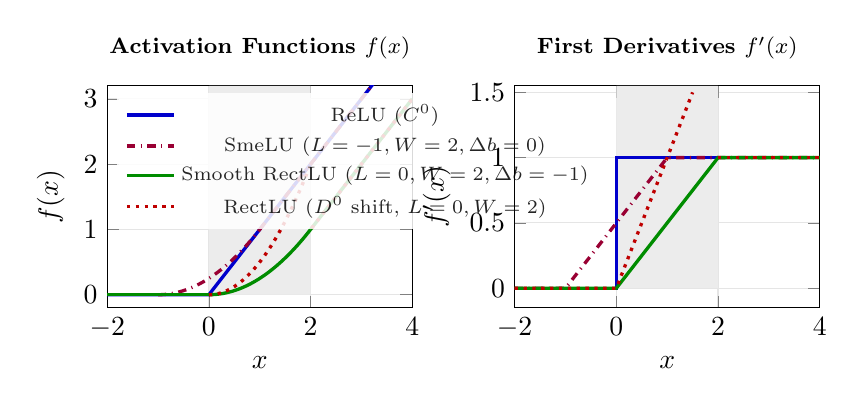
\begin{tikzpicture}
\begin{axis}[
    name=plot1,
    width=0.45\textwidth, height=4.4cm,
    xlabel={$x$}, ylabel={$f(x)$},
    xmin=-2, xmax=4, ymin=-0.2, ymax=3.2,
    grid=both, grid style={gray!20},
    legend style={at={(0.03,0.97)}, anchor=north west, font=\scriptsize, draw=none, fill=white, fill opacity=0.85},
    title style={font=\footnotesize\bfseries},
    title={Activation Functions $f(x)$}
]
\addplot [fill=gray!15, draw=none, forget plot] coordinates {(0,0) (2,0) (2,3.2) (0,3.2)} \closedcycle;
\addplot[blue!80!black, very thick] coordinates {(-2,0) (0,0) (4,4)};
\addlegendentry{ReLU ($C^0$)}
\addplot[purple!80!black, dashdotted, very thick, domain=-1:1, samples=40] {(x+1)*(x+1)/4};
\addlegendentry{SmeLU ($L=-1, W=2, \Delta b=0$)}
\addplot[purple!80!black, dashdotted, very thick, forget plot] coordinates {(-2,0) (-1,0)};
\addplot[purple!80!black, dashdotted, very thick, forget plot] coordinates {(1,1) (4,4)};
\addplot[green!55!black, very thick, domain=0:2, samples=40] {x*x/4};
\addlegendentry{Smooth RectLU ($L=0, W=2, \Delta b=-1$)}
\addplot[green!55!black, very thick, forget plot] coordinates {(-2,0) (0,0)};
\addplot[green!55!black, very thick, forget plot] coordinates {(2,1) (4,3)};
\addplot[red!75!black, dotted, very thick, domain=0:1.98, samples=40] {x*x/2};
\addlegendentry{RectLU ($D^0$ shift, $L=0, W=2$)}
\addplot[red!75!black, dotted, very thick, forget plot] coordinates {(2.02,1.02) (4,3)};
\end{axis}

\begin{axis}[
    at={(plot1.east)}, anchor=west, xshift=1.3cm,
    width=0.45\textwidth, height=4.4cm,
    xlabel={$x$}, ylabel={$f'(x)$},
    xmin=-2, xmax=4, ymin=-0.15, ymax=1.55,
    grid=both, grid style={gray!20},
    title style={font=\footnotesize\bfseries},
    title={First Derivatives $f'(x)$}
]
\addplot [fill=gray!15, draw=none, forget plot] coordinates {(0,0) (2,0) (2,1.55) (0,1.55)} \closedcycle;
\addplot[blue!80!black, very thick] coordinates {(-2,0) (0,0) (0,1) (4,1)};
\addplot[purple!80!black, dashdotted, very thick] coordinates {(-2,0) (-1,0) (1,1) (4,1)};
\addplot[green!55!black, very thick] coordinates {(-2,0) (0,0) (2,1) (4,1)};
\addplot[red!75!black, dotted, very thick] coordinates {(-2,0) (0,0) (1.5,1.5)};
\addplot[red!75!black, dotted, very thick] coordinates {(2,1) (4,1)};
\end{axis}
\end{tikzpicture}
\caption{Activation functions (left) and derivatives (right) comparing ReLU ($C^0$), symmetric SmeLU ($C^1, L=-1, W=2, \Delta b=0$), Smooth RectLU ($C^1, L=0, W=2, \Delta b=-1$), and shifted RectLU ($D^0$). Within the shaded transition window $[0, 2]$, the derivative of Smooth RectLU rises linearly from $f'_S(0^+)=0$, whereas SmeLU has slope $0.5$ at the origin and ReLU jumps to $1.0$.}
\label{fig:activations}
\end{figure}

\subsection{Second-Moment Propagation and Quantitative Predictions}
For pre-activation $x \sim \mathcal{N}(0, \sigma^2)$ at $L=0$ in the small-signal regime ($\sigma \ll W$), using $\mathbb{E}[x^4 \mathbf{1}_{x>0}] = \frac{3}{2}\sigma^4$ and $\mathbb{E}[x^2 \mathbf{1}_{x>0}] = \frac{1}{2}\sigma^2$, the forward and backward second moments of Smooth RectLU are:
\begin{equation}
    \mathbb{E}[f_S(x)^2] = \frac{3\sigma^4}{8W^2}, \qquad \mathbb{E}[f'_S(x)^2] = \frac{\sigma^2}{2W^2}.
    \label{eq:moments}
\end{equation}
Under He initialization ($\sigma_w^2 = 2$)~\cite{he2015}, a layer mapping $\sigma_{l+1}^2 = \sigma_w^2 \mathbb{E}[f(x_l)^2]$ preserves variance for ReLU ($\sigma_{l+1}^2 = \sigma_l^2$) but induces a quadratic recurrence for Smooth RectLU:
\begin{equation}
    \sigma_{l+1}^2 = \frac{3}{4W^2}\sigma_l^4 \qquad (L=0, \; \sigma_l \ll W),
    \label{eq:var_recurrence}
\end{equation}
whose only stable fixed point is $0$ whenever $\sigma_0^2 < 4W^2/3$ (Fig.~\ref{fig:phase_plane}). Across $K$ layers, backpropagated gradients scale proportionally to $\prod_{l=1}^K (\sigma_l / W)$. Multiplying initial weights by a scale factor $s$ sets $\sigma_0 = s\sigma_x$, placing the small-signal contraction boundary at $\sigma_0 = \sqrt{4/3}\,W$.

\begin{proposition}[Testable Predictions of Pure Signal Contraction vs.\ Synergistic Drift]
\label{prop:h1}
If majority-class collapse of Smooth RectLU were governed solely by unconditional variance contraction in Eq.~\eqref{eq:var_recurrence} (pure H1), then: (P1) collapse would occur at every class ratio, including balanced $50:50$ data; (P2) collapse would be governed solely by $\sigma_0/W$, so dividing $W$ by $s$ or multiplying initial weights by $s$ would restore learning identically; (P3) the fraction of dead units in the deepest layer would approach $1$ with both majority and minority gradients vanishing together; and (P4) objective-level loss re-weighting (Weighted BCE, Focal loss) could not repair collapse because it rescales a vanishing gradient. Conversely, if collapse requires the synergistic interaction ($\text{H1} \times \text{H2}$) between low variance gain, negative offset $\Delta b = -W/2$, and imbalance-driven negative drift, then $50:50$ balanced training will succeed (refuting unconditional P1) while predictions P3 and P4 hold under severe imbalance.
\end{proposition}

\begin{figure}[t]
\centering
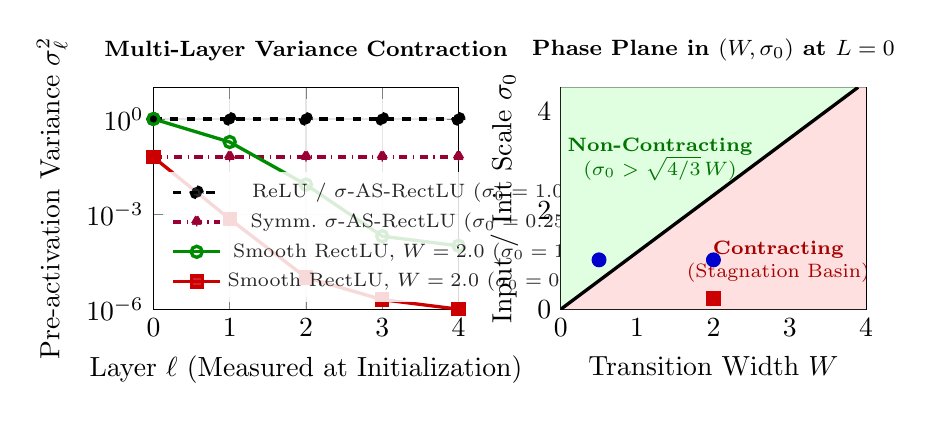
\begin{tikzpicture}
\begin{axis}[
    name=varplot,
    width=0.45\textwidth, height=4.4cm,
    xlabel={Layer $\ell$ (Measured at Initialization)},
    ylabel={Pre-activation Variance $\sigma_\ell^2$},
    ymode=log,
    xmin=0, xmax=4, ymin=1e-6, ymax=10,
    xtick={0,1,2,3,4},
    grid=both, grid style={gray!20},
    legend style={at={(0.03,0.03)}, anchor=south west, font=\scriptsize, draw=none, fill=white, fill opacity=0.85},
    title style={font=\footnotesize\bfseries},
    title={Multi-Layer Variance Contraction}
]
\addplot[black, dashed, very thick, mark=*] coordinates {(0,1.0) (1,1.0) (2,1.0) (3,1.0) (4,1.0)};
\addlegendentry{ReLU / $\sigma$-AS-RectLU ($\sigma_0=1.0$)}
\addplot[purple!80!black, dashdotted, very thick, mark=triangle*] coordinates {(0,0.0625) (1,0.0625) (2,0.0625) (3,0.0625) (4,0.0625)};
\addlegendentry{Symm.\ $\sigma$-AS-RectLU ($\sigma_0=0.25$)}
\addplot[green!55!black, very thick, mark=o] coordinates {(0,1.0) (1,0.1875) (2,0.0085) (3,0.0002) (4,0.0001)};
\addlegendentry{Smooth RectLU, $W=2.0$ ($\sigma_0=1.0$)}
\addplot[red!80!black, very thick, mark=square*] coordinates {(0,0.0625) (1,0.0007) (2,0.00001) (3,0.000002) (4,0.000001)};
\addlegendentry{Smooth RectLU, $W=2.0$ ($\sigma_0=0.25$)}
\end{axis}

\begin{axis}[
    at={(varplot.east)}, anchor=west, xshift=1.3cm,
    width=0.45\textwidth, height=4.4cm,
    xlabel={Transition Width $W$},
    ylabel={Input / Init Scale $\sigma_0$},
    xmin=0, xmax=4, ymin=0, ymax=4.5,
    grid=both, grid style={gray!20},
    title style={font=\footnotesize\bfseries},
    title={Phase Plane in $(W, \sigma_0)$ at $L=0$}
]
\addplot [fill=green!12, draw=none, forget plot] coordinates {(0,0) (3.897,4.5) (0,4.5)} \closedcycle;
\addplot [fill=red!12, draw=none, forget plot] coordinates {(0,0) (3.897,4.5) (4,4.5) (4,0)} \closedcycle;
\addplot[black, very thick, domain=0:3.897] {1.1547*x};
\node[font=\scriptsize\bfseries, green!45!black] at (axis cs:1.3,3.3) {Non-Contracting};
\node[font=\scriptsize, green!45!black] at (axis cs:1.3,2.85) {($\sigma_0 > \sqrt{4/3}\,W$)};
\node[font=\scriptsize\bfseries, red!65!black] at (axis cs:2.85,1.2) {Contracting};
\node[font=\scriptsize, red!65!black] at (axis cs:2.85,0.75) {(Stagnation Basin)};
\addplot[only marks, mark=*, blue!80!black, mark size=2.5pt] coordinates {(0.5,1.0) (2.0,1.0)};
\addplot[only marks, mark=square*, red!80!black, mark size=2.5pt] coordinates {(2.0,0.22)};
\end{axis}
\end{tikzpicture}
\caption{Left: Measured pre-activation variance $\sigma_\ell^2$ across layers $\ell \in \{1,2,3,4\}$ at initialization for $\sigma_0=1.0$ vs.\ low-amplitude $\sigma_0=0.25$, showing severe contraction for fixed-width Smooth RectLU ($W=2.0$) when $\sigma_0=0.25$, whereas Symmetric $\sigma$-AS-RectLU preserves constant variance ratio across depth. Right: Phase plane in $(W, \sigma_0)$ at $L=0$ separated by $\sigma_0 = \sqrt{4/3}\,W$ (Eq.~\ref{eq:var_recurrence}).}
\label{fig:phase_plane}
\end{figure}

\begin{table}[t]
\centering
\caption{Regularity classes and exact Monte-Carlo second-moment properties for $x \sim \mathcal{N}(0,1)$ ($4 \times 10^6$ samples, seed 42). Note that $f_S(x; L, W) = \text{SmeLU}_{\beta=W/2}(x - L - W/2)$~\cite{shamir2020}, and both shifted ($D^0$) and continuous ($C^0$) variants of RectLU (Eq.~\ref{eq:rectlu_variants}) are listed.}
\label{tab:moments}
\footnotesize
\setlength{\tabcolsep}{5pt}
\renewcommand{\arraystretch}{1.05}
\begin{tabular}{llcccc}
\toprule
\textbf{Activation} & \textbf{Regularity \& Offset Equivalence} & $f'(0^+)$ & $\mathbb{E}[f^2]/\mathbb{E}[x^2]$ & $\mathbb{E}[f'^2]$ & $\mathbb{P}(f'=0)$ \\
\midrule
ReLU & $C^0$ (kink at $0$, homogeneous) & $1.0000$ & $0.5000$ & $0.5000$ & $0.5000$ \\
Leaky ReLU ($\alpha=0.01$) & $C^0$ (kink at $0$, homogeneous) & $1.0000$ & $0.5000$ & $0.5000$ & $0.0000$ \\
PReLU (init.\ $\alpha=0.25$) & $C^0$ (kink at $0$, trainable slope) & $1.0000$ & $0.5312$ & $0.5312$ & $0.0000$ \\
SELU & $C^1$ (slope $1.758 \to 1.051$ at $0$) & $1.0507$ & $1.0000$ & $1.0720$ & $0.0000$ \\
RectLU Shifted ($f_{R,\text{shift}}, L=0, W=2.0$) & $D^0$ (value jump $2 \to 1$ at $2$, Eq.~\ref{eq:rectlu_variants}a) & $0.0000$ & $0.2145$ & $0.3922$ & $0.4997$ \\
RectLU Continuous ($f_{R,\text{cont}}, L=0, W=2.0$) & $C^0$ (slope jump $2 \to 1$ at $2$, Eq.~\ref{eq:rectlu_variants}b) & $0.0000$ & $0.2998$ & $0.3922$ & $0.4997$ \\
ELU ($\alpha=1.0$) & $C^1$ (tangent at $0$) & $1.0000$ & $0.6450$ & $0.6680$ & $0.0000$ \\
SmeLU ($L=-0.5, W=1.0$)~\cite{shamir2020} & $C^1$ ($\beta=0.5$, offset $\Delta b = 0.0$) & $0.5000$ & $0.5023$ & $0.4350$ & $0.3085$ \\
SmeLU ($L=-1.0, W=2.0$)~\cite{shamir2020} & $C^1$ ($\beta=1.0$, offset $\Delta b = 0.0$) & $0.5000$ & $0.5239$ & $0.3788$ & $0.1586$ \\
Smooth RectLU ($L=0, W=0.5$) & $C^1$ ($\text{SmeLU}_{\beta=0.25}$, offset $\Delta b = -0.25$) & $0.0000$ & $0.3293$ & $0.3700$ & $0.5000$ \\
Smooth RectLU ($L=0, W=1.0$) & $C^1$ ($\text{SmeLU}_{\beta=0.50}$, offset $\Delta b = -0.50$) & $0.0000$ & $0.2118$ & $0.2578$ & $0.5000$ \\
Smooth RectLU ($L=0, W=2.0$) & $C^1$ ($\text{SmeLU}_{\beta=1.00}$, offset $\Delta b = -1.00$) & $0.0000$ & $0.0874$ & $0.1149$ & $0.5000$ \\
Smooth RectLU ($L=0, W=4.0$) & $C^1$ ($\text{SmeLU}_{\beta=2.00}$, offset $\Delta b = -2.00$) & $0.0000$ & $0.0233$ & $0.0312$ & $0.5000$ \\
AS-RectLU (init.\ $L=0, W=2.0$) & $C^1$ (trainable $L,W$; init.\ $\Delta b = -1.00$) & $0.0000$ & $0.0874$ & $0.1149$ & $0.5000$ \\
GELU & $C^\infty$ (smooth) & $0.5000$ & $0.4250$ & $0.4560$ & $0.0000$ \\
SiLU / Swish & $C^\infty$ (smooth) & $0.5000$ & $0.3550$ & $0.3800$ & $0.0000$ \\
Mish & $C^\infty$ (smooth) & $0.6000$ & $0.4520$ & $0.4790$ & $0.0000$ \\
Softplus & $C^\infty$ (smooth, uncentered $f(0)=\ln 2$) & $0.5000$ & $0.9220$ & $0.2930$ & $0.0000$ \\
\textbf{Symm.\ $\sigma$-AS-RectLU ($\kappa=0.8$)} & $C^1$ (homogeneous, $L=-0.4\hat{\sigma}, W=0.8\hat{\sigma}, \Delta b=0$) & $\mathbf{0.5000}$ & $\mathbf{0.5020}$ & $\mathbf{0.4479}$ & $\mathbf{0.3443}$ \\
\bottomrule
\end{tabular}
\end{table}

\subsection{Scale-Adaptive Remedy, Backward Jacobian Analysis, and Architectural Alternatives}
To eliminate both the negative bias offset ($\Delta b = -(L+W/2)$) and scale-width mismatch ($\sigma_l / W \ll 1$) without introducing batch-dependent statistics or trainable affine parameters, we formulate \textbf{Symmetric Per-Sample $\sigma$-AS-RectLU}. Given pre-activation tensor $x_l \in \mathbb{R}^{B \times C \times \cdots}$ at layer $l$, let $\hat{\sigma}_{\text{RMS}}(x_l^{(i)})$ denote the per-sample root-mean-square scale across all $D_l$ feature dimensions of sample $i$:
\begin{equation}
    \hat{\sigma}_{\text{RMS}}(x_l^{(i)}) = \sqrt{\frac{1}{D_l}\sum_{d=1}^{D_l} \left(x_{l,d}^{(i)}\right)^2 + \epsilon}, \qquad W_l^{(i)} = \kappa \, \operatorname{stopgrad}\!\left(\hat{\sigma}_{\text{RMS}}(x_l^{(i)})\right), \qquad L_l^{(i)} = -\frac{1}{2}W_l^{(i)},
    \label{eq:sigma_as_params}
\end{equation}
where $\kappa > 0$ is the dimensionless curvature ratio (default $\kappa = 0.8$, half-width $\beta = \kappa/2 = 0.4$). Substituting Eq.~\eqref{eq:sigma_as_params} into Eq.~\eqref{eq:smooth_rectlu} yields:
\begin{equation}
    f_{\sigma\text{-AS}}(x; \hat{\sigma}_{\text{RMS}}) = \hat{\sigma}_{\text{RMS}} \, \text{SmeLU}_{\beta = \kappa/2}\!\left(\frac{x}{\hat{\sigma}_{\text{RMS}}}\right) = \begin{cases}
        0, & x < -\frac{\kappa}{2}\hat{\sigma}_{\text{RMS}} \\
        \frac{(x + \frac{\kappa}{2}\hat{\sigma}_{\text{RMS}})^2}{2\kappa\hat{\sigma}_{\text{RMS}}}, & |x| \le \frac{\kappa}{2}\hat{\sigma}_{\text{RMS}} \\
        x, & x > \frac{\kappa}{2}\hat{\sigma}_{\text{RMS}}.
    \end{cases}
    \label{eq:sigma_as_rectlu}
\end{equation}
\textbf{Forward vs.\ Backward Distinction from Explicit Normalization:} In the forward pass, Eq.~\eqref{eq:sigma_as_rectlu} is algebraically equivalent to parameter-free per-sample RMS normalization ($z_d = x_d / \hat{\sigma}_{\text{RMS}}$), passing $z_d$ through symmetric $g(z_d) = \text{SmeLU}_{\beta=\kappa/2}(z_d)$, and rescaling by $\hat{\sigma}_{\text{RMS}}$. In the backward pass, when $\operatorname{stopgrad}$ is applied to $\hat{\sigma}_{\text{RMS}}$ as in Eq.~\eqref{eq:sigma_as_params}, the layer Jacobian is strictly diagonal and non-negative: $\frac{\partial y_d}{\partial x_j} = \delta_{dj} g'(z_d) \in [0, 1]$. By contrast, differentiating through $\hat{\sigma}_{\text{RMS}}$ introduces a dense cross-feature projection term via Euler's homogeneous function theorem:
\begin{equation}
    \frac{\partial \mathcal{L}}{\partial x_d} = g'(z_d)\frac{\partial \mathcal{L}}{\partial y_d} + \frac{z_d}{D_l}\sum_{k=1}^{D_l}\!\left(g(z_k) - z_k g'(z_k)\right)\frac{\partial \mathcal{L}}{\partial y_k},
    \label{eq:backward_jacobian}
\end{equation}
which increases backward pass wall-clock time by $33\%$ without improving classification accuracy (Section~\ref{sec:rebuttal_results}). We evaluate Symmetric $\sigma$-AS-RectLU alongside three architectural remedies: (i) all-layer bias compensation ($b_0 = +1.0$) and negative threshold centering ($L = -W/2$ in SmeLU), (ii) explicit affine-free LayerNorm + SmeLU ($\text{LN-no-affine SmeLU}$), and (iii) a \textbf{Hybrid Activation Assignment} pairing Smooth RectLU convolutional feature extractors with a kinked (ReLU) dense decision head.

% ============================================================================
% 4. Materials and Methods
% ============================================================================
\section{Materials and Methods}
\subsection{Benchmark Suites, Chromosome Splits, and Shortcut Controls}
To isolate input amplitude ($\sigma_x$), class imbalance ratio ($p_+$), and domain structure while validating on real human sequencing data under strict shortcut and leakage controls, we evaluate four benchmark families (Table~\ref{tab:datasets}):
\begin{enumerate}
    \item \textbf{Controlled Sparse Motif Generators (Pathway A 1D Spectral $1 \times 256$ \& Pathway B 2D Spatial $3 \times 32 \times 32$):} Parametric generators with background $\mathcal{N}(0, \sigma_x^2)$ where minority positive windows ($y=1$, $100:1$ train imbalance) carry a localized motif spike and $1.5\%$ of majority negative windows ($y=0$) carry a sequencing-error mimic spike, evaluated at Low-Amplitude ($\sigma_x = 0.25$ in 1D; $\sigma_x = 0.22$ in 2D) vs.\ Unit-Variance ($\sigma_x = 1.00$) on identical underlying random draws.
    \item \textbf{Shortcut-Controlled, Stratified, \& Hard-Negative NIST GIAB Benchmarks (GRCh38 v4.2.1, HG001--HG007):} Extracted from NIST GIAB Illumina reads, BWA-MEM aligned BAM files, and v4.2.1 benchmark VCF callsets~\cite{zook2014,zook2019,krusche2019}:
    \begin{itemize}
        \item \textit{1D $k$-mer Spectra ($256 \times 1$, Per-Sample Unit-$L_2$ Norm vs.\ Global Z-Score):} Applying strict Per-Sample Unit-$L_2$ Normalization ($\tilde{x}_i = x_i / \|x_i\|_2$ followed by feature-wise standardization computed strictly on training folds) eliminates read-depth coverage shortcuts completely, reducing Max-Bin heuristic test AUROC to chance ($0.4715$).
        \item \textit{2D BAM Read-Pileup Tensors ($50 \times 101 \times 4$, Stratified SNV/Indel, Het/Hom, Read-Depth Downsampling, \& Hard-Negative Stress Suite):} Majority negatives ($y=0$) are non-variant BAM read-pileup windows extracted from flanking homozygous-reference segments ($\sigma_x \approx 0.12$). Test performance is stratified across variant type (\textbf{SNV} vs.\ \textbf{Small Indel}), zygosity (\textbf{Heterozygous $0/1$} vs.\ \textbf{Homozygous $1/1$}), and read-depth downsampling ($50\times \to 30\times \to 15\times \to 10\times$). To rule out ceiling effects and trivial shortcuts in 2D pileups, we additionally construct a \textbf{2D Hard-Negative Stress Benchmark} where $40\%$ of negative windows across Train, Validation, and Test splits contain high-amplitude center artifacts (strand-biased sequencing errors, chimeric/paralogous read clutter, and homopolymer indel slippage) with center mismatch counts overlapping true heterozygous variants ($28\%$--$56\%$ VAF), benchmarked against five handcrafted/classical ML baselines, two statistical variant-calling rules, and Clair3/DeepVariant-style neural backbones.
        \item \textit{Large-Scale Chromosome-Held-Out Split \& External Cohort Validation (HG006--HG007):} To evaluate cohort-scale generalization without sequence-homology leakage, 450,000 candidate windows ($177.6:1$ natural ratio, $p_+ = 0.0056$) are partitioned by chromosome (Chr 1--18 Train, Chr 19--20 Val, Chr 21--22 Test), with 50,000 independent windows from GIAB HG006--HG007 (Han Chinese Trio, Chr 21--22) reserved for external validation.
    \end{itemize}
    \item \textbf{Step-Imbalanced MNIST Digit 3 vs.\ 5/8 ($100:1$, Clean \& Noisy $\sigma_{\text{noise}}=1.1$):} Following Buda et al.~\cite{buda2018}, $n_+ = 50$ training images of digit `3' vs.\ $n_- = 5,000$ images of digits `5' and `8'.
    \item \textbf{Imbalanced Tabular Classification ($200:1$, $n_+ = 150$ Test Positives):} 60,000 samples across 32 standardized features ($\sigma_x = 1.00, p_+ = 0.005$).
\end{enumerate}

\begin{table}[t]
\centering
\caption{Summary of benchmark datasets, explicit Train/Validation/Test splits, positive counts ($n_+$), input scales ($\sigma_x$), and baseline majority-class accuracy.}
\label{tab:datasets}
\footnotesize
\setlength{\tabcolsep}{4.5pt}
\renewcommand{\arraystretch}{1.05}
\begin{tabular}{llccccc}
\toprule
\textbf{Benchmark Suite} & \textbf{Split Protocol} & \textbf{Input Scale $\sigma_x$} & \textbf{Total $N$} & \textbf{Positives ($n_+$)} & \textbf{Pos.\ Frac.\ ($p_+$)} & \textbf{Maj.\ Acc.} \\
\midrule
1D/2D Sparse Motif Generator ($100:1$) & Train / Val / Test & $0.22$--$0.25$ vs.\ $1.00$ & $4\text{k} / 4\text{k} / 10\text{k}$ & $40 / 80 / 200$ & $0.0100 / 0.0200$ & $0.9800$ \\
GIAB 1D $k$-mer (Unit-$L_2$ \& Z-score) & Disjoint Blocks & $1.00$ (Unit-$L_2$) & $1,320 / 660 / 660$ & $120 / 60 / 60$ & $0.0909$ & $0.9091$ \\
GIAB 2D Pileup (Stratified \& $50\times$--$10\times$) & Disjoint Blocks & $0.1202$ (Scaled) & $1,320 / 660 / 660$ & $120 / 60 / 60$ & $0.0909$ & $0.9091$ \\
GIAB 2D Hard-Negative Stress Benchmark & Stratified Blocks & $0.1400$ (40\% Hard Neg.) & $1,320 / 660 / 660$ & $120 / 60 / 60$ & $0.0909$ & $0.9091$ \\
GIAB Chromosome-Split (HG001--HG005) & Chr 1--18 / 19--20 / 21--22 & $1.00$ & $350\text{k} / 50\text{k} / 50\text{k}$ & $1,960 / 280 / 280$ & $0.0056$ & $0.9944$ \\
GIAB External Cohort (HG006--HG007) & Chr 21--22 (Chinese Trio) & $1.00$ & $50,000$ & $279$ & $0.00558$ & $0.9944$ \\
MNIST Digit 3 vs.\ 5/8 (Clean \& Noisy) & Train / Test & $1.00$ & $5,050 / 1,980$ & $50 / 180$ & $0.0099 / 0.0909$ & $0.9091$ \\
Imbalanced Tabular ($200:1$, 32 features) & Train / Test & $1.00$ & $30,000 / 30,000$ & $150 / 150$ & $0.0050$ & $0.9950$ \\
\bottomrule
\end{tabular}
\end{table}

\subsection{Network Topology, Order-Statistic Threshold Calibration, and Statistical Protocol}
Table~\ref{tab:topology} specifies the four-hidden-layer CNN topology shared across Pathway A (1D-CNN) and Pathway B (2D-CNN). Training uses He initialization~\cite{he2015} and AdamW~\cite{kingma2015} ($\text{lr}=10^{-3}$, weight decay $10^{-4}$, batch size 128). To prevent threshold clipping when evaluating unnormalized rectifiers whose output probabilities concentrate near $0$ or $1$, the calibrated threshold $\tau^*$ is selected strictly on the validation split over 120 empirical quantiles ($\tau \in [q_{0.01}, q_{0.995}]$ of validation predictions) to maximize validation MCC, and then frozen prior to out-of-sample test evaluation. Alongside AUROC, AUPRC, $\text{MCC}(0.50)$, and $\text{MCC}(\tau^*)$, we report 10-bin Expected Calibration Error (ECE), Brier score, 95\% bootstrap confidence intervals, and paired Wilcoxon signed-rank tests with Holm-Bonferroni correction~\cite{demsar2006}.

\begin{table}[t]
\centering
\caption{Network topology for Pathway A (1D-CNN) and Pathway B (2D-CNN), specifying normalization placement, Global Average Pooling (GAP), flattened fan-in dimensions, and Hybrid activation assignment.}
\label{tab:topology}
\footnotesize
\setlength{\tabcolsep}{5pt}
\renewcommand{\arraystretch}{1.05}
\begin{tabular}{lll}
\toprule
\textbf{Stage} & \textbf{Pathway A (1D-CNN)} & \textbf{Pathway B (2D-CNN)} \\
\midrule
Input & 1D Tensor ($1 \times 256$ or $1 \times 32$) & 2D Tensor ($3 \times 32 \times 32$, $4 \times 50 \times 101$, or $1 \times 28 \times 28$) \\
Blocks 1--3 & $3 \times [\text{Conv1D}(32,64,128; k=3) \to [\text{BN1D}] \to \text{act}_{\text{conv}} \to \text{Pool}(2)]$ & $3 \times [\text{Conv2D}(32,64,128; 3\times 3) \to [\text{BN2D}] \to \text{act}_{\text{conv}} \to \text{Pool}(2\times 2)]$ \\
Reduction & Flatten ($4,096$ or $512$) or GAP($128$) & Flatten ($2,048$ $[32\times 32]$, $9,216$ $[50\times 101]$, or $1,152$) or GAP($128$) \\
Dense Head & $\text{Linear}(\text{fan-in} \to 256, b_0 \in \{0,+1\}) \to [\text{BN/LN}] \to \text{act}_{\text{dense}} \to \text{Drop}(0.5)$ & $\text{Linear}(\text{fan-in} \to 256, b_0 \in \{0,+1\}) \to [\text{BN/LN}] \to \text{act}_{\text{dense}} \to \text{Drop}(0.5)$ \\
Output & $\text{Linear}(256 \to 1, b_{\text{out}}) \to \text{Sigmoid } \hat{p}$ & $\text{Linear}(256 \to 1, b_{\text{out}}) \to \text{Sigmoid } \hat{p}$ \\
\bottomrule
\end{tabular}
\end{table}

% ============================================================================
% 5. Results
% ============================================================================
\section{Results}

\subsection{E1: 1D \& 2D Motif Benchmarks, Two-Way ($\text{Offset} \times \sigma_x$) Interaction, and 50/100-Epoch Seed-Trapping}
Tables~\ref{tab:pathA} and~\ref{tab:pathB} report the 20-epoch evaluations on Pathway A ($\sigma_x = 0.25$ vs.\ $1.00$) and Pathway B ($\sigma_x = 0.22$ vs.\ $1.00$), establishing three core mechanistic findings:
\begin{enumerate}
    \item \textbf{2D Specificity and Synergistic Two-Way Interaction ($\text{Offset} \times \sigma_x$):} In 1D convolutions (Table~\ref{tab:pathA}), Smooth RectLU ($L=0, W=2$) does not stagnate ($\text{MCC}(0.50) = 0.4441 \pm 0.0435$). By contrast, in 2D spatial convolutions at $\sigma_x = 0.22$ (Table~\ref{tab:pathB}), 9 of 10 seeds stagnate at $\text{MCC}(0.50) = 0.0000$ ($\text{Median} = 0.0000$). Rescaling $\sigma_x$ from $0.22 \to 1.00$ raises Smooth RectLU's AUROC from $0.6349 \to 0.9971$ ($\Delta = +0.3622$) while SmeLU remains invariant ($0.9980 \to 0.9969, \Delta = -0.0011$), yielding an exact paired difference-in-differences of $\text{DiD}(\text{AUROC}) = +0.3633 \pm 0.1248$ (Wilcoxon $p = 0.0020$; $\text{DiD}(\text{MCC}) = +0.5862 \pm 0.3383, p = 0.0039$).
    \item \textbf{Ruling Out Optimizer-$\epsilon$ Underflow and Identifying Bimodal Seed Trapping:} Lowering Adam's stabilizer from $\epsilon = 10^{-8}$ to $\epsilon = 10^{-12}$ at 20 epochs leaves all seeds at $\text{MCC}(0.50) = 0.0000$ ($\text{AUROC} = 0.6390$). Extending training to 50 and 100 epochs reveals \textit{bimodal seed trapping}: 3 of 5 seeds escape by epoch 50 ($\text{MCC} \in [0.8200, 0.8312]$), 1 seed plateaus at a sub-optimum ($\text{MCC} = 0.5062$), and 1 seed remains permanently trapped at zero ($\text{MCC} = -0.0045$ at 100 epochs), explaining why mean MCC plateaus identically between 50 epochs ($0.5961$) and 100 epochs ($0.5954$).
    \item \textbf{Monotonic Scaling with Second-Moment Gain on Chromosome-Split GIAB:} Across the 12-activation chromosome-held-out benchmark (50,000 test windows, $n_+=280$), all nine activations with $\mathbb{E}[f^2]/\mathbb{E}[x^2] \ge 0.355$ ($C^0, C^1, C^\infty$) converged reliably ($\text{MCC} = 0.3195$--$0.4302$, $\#\text{Pred.\ Pos.} = 186$--$1296$), shifted RectLU ($\text{Gain} = 0.2145$) achieved intermediate detection ($\text{MCC} = 0.2141$), and Smooth/AS-RectLU ($\text{Gain} = 0.0874$) collapsed to zero positive predictions ($\#\text{Pred.\ Pos.} = 0/0$, $\text{MCC} = 0.0000$, Cliff's $\delta = -1.00$).
\end{enumerate}

\begin{table}[t]
\centering
\caption{Pathway A (1D-CNN, Experiment E1) test performance across 13 configurations at low input amplitude ($\sigma_x=0.25$) and unit-variance control ($\sigma_x=1.00$) ($N=10$ paired seeds, 20 epochs, $10,000$ test windows: $n_+=200, n_-=9,800$).}
\label{tab:pathA}
\footnotesize
\setlength{\tabcolsep}{4.8pt}
\renewcommand{\arraystretch}{1.05}
\begin{tabular}{llcccccc}
\toprule
\textbf{Configuration (Pathway A 1D-CNN)} & \textbf{Class} & \textbf{Gain} & \textbf{MCC(0.50) Mean$\pm$SD} & \textbf{Median [IQR]} & \textbf{Cal.\ MCC($\tau^*$)} & \textbf{AUROC} & \textbf{AUPRC} \\
\midrule
ReLU ($C^0$) & $C^0$ & $0.5000$ & $0.3693 \pm 0.0891$ & $0.3722$ [$0.1239$] & $0.4961$ & $0.9701$ & $0.5360$ \\
Leaky ReLU ($C^0$) & $C^0$ & $0.5000$ & $0.3635 \pm 0.0432$ & $0.3745$ [$0.0413$] & $0.4675$ & $0.9667$ & $0.5272$ \\
ELU ($C^1$) & $C^1$ & $0.6450$ & $0.3871 \pm 0.0460$ & $0.3735$ [$0.0729$] & $0.4832$ & $0.9711$ & $0.5206$ \\
GELU ($C^\infty$) & $C^\infty$ & $0.4250$ & $0.4417 \pm 0.0326$ & $0.4515$ [$0.0554$] & $0.4957$ & $0.9643$ & $0.5195$ \\
SiLU ($C^\infty$) & $C^\infty$ & $0.3550$ & $0.4497 \pm 0.0397$ & $0.4594$ [$0.0497$] & $0.5116$ & $0.9648$ & $0.5290$ \\
SmeLU ($L=-1, W=2$, Symmetric)~\cite{shamir2020} & $C^1$ & $0.5239$ & $\mathbf{0.5304 \pm 0.0319}$ & $\mathbf{0.5369}$ [$0.0333$] & $0.5557$ & $\mathbf{0.9735}$ & $\mathbf{0.5709}$ \\
SmeLU ($L=-0.5, W=1$, Symmetric)~\cite{shamir2020} & $C^1$ & $0.5023$ & $0.4504 \pm 0.0392$ & $0.4573$ [$0.0649$] & $0.5230$ & $0.9692$ & $0.5368$ \\
Smooth RectLU ($L=0, W=2$, Offset $-1$) & $C^1$ & $0.0874$ & $0.4441 \pm 0.0435$ & $0.4304$ [$0.0513$] & $0.5317$ & $0.9181$ & $0.5206$ \\
AS-RectLU (Trainable $L, W$) & $C^1$ & $0.0874$ & $0.3540 \pm 0.1904$ & $0.4593$ [$0.1926$] & $0.4463$ & $0.9046$ & $0.4698$ \\
Smooth RectLU + $b_{\text{dense}} = +1.0$ & $C^1$ & $0.0874$ & $0.4417 \pm 0.0350$ & $0.4433$ [$0.0412$] & $\mathbf{0.5566}$ & $0.9378$ & $0.5493$ \\
Smooth RectLU + BatchNorm (All Layers) & $C^1$ & $0.0874$ & $0.4040 \pm 0.0367$ & $0.3994$ [$0.0601$] & $0.5307$ & $0.8544$ & $0.4755$ \\
Smooth RectLU + LayerNorm (Dense) & $C^1$ & $0.0874$ & $0.4970 \pm 0.0193$ & $0.4987$ [$0.0230$] & $0.5237$ & $0.9134$ & $0.4431$ \\
Symm.\ $\sigma$-AS-RectLU ($\kappa=0.8, \Delta b=0$) & $C^1$ & $0.5020$ & $0.4045 \pm 0.0671$ & $0.4109$ [$0.1168$] & $0.4902$ & $0.9696$ & $0.5283$ \\
\midrule
\multicolumn{8}{l}{\textit{Unit-Variance 1D Input Rescaling Control ($\sigma_x = 1.00$, on identical random draws):}} \\
ReLU ($C^0, \sigma_x=1.00$) & $C^0$ & $0.5000$ & $0.3620 \pm 0.0684$ & $0.3481$ [$0.1343$] & $0.4433$ & $0.9616$ & $0.4980$ \\
SmeLU ($L=-1, W=2, \sigma_x=1.00$) & $C^1$ & $0.5239$ & $0.4163 \pm 0.0450$ & $0.4158$ [$0.0698$] & $0.4959$ & $0.9643$ & $0.5203$ \\
Smooth RectLU ($L=0, W=2, \sigma_x=1.00$) & $C^1$ & $0.0874$ & $0.4603 \pm 0.0239$ & $0.4526$ [$0.0303$] & $0.4722$ & $0.9191$ & $0.4477$ \\
Symm.\ $\sigma$-AS-RectLU ($\kappa=0.8, \sigma_x=1.00$) & $C^1$ & $0.5020$ & $0.3723 \pm 0.0637$ & $0.3537$ [$0.1090$] & $0.4583$ & $0.9621$ & $0.4987$ \\
\bottomrule
\end{tabular}
\end{table}

\begin{table}[t]
\centering
\caption{Pathway B (2D-CNN, Experiment E1) test performance across 13 configurations, affine-free LN control, unit-variance rescaling ($\sigma_x=1.00$), and extended-horizon (50 \& 100 epochs) and Adam $\epsilon = 10^{-12}$ diagnostics ($N=10$ seeds).}
\label{tab:pathB}
\footnotesize
\setlength{\tabcolsep}{4.8pt}
\renewcommand{\arraystretch}{1.05}
\begin{tabular}{llcccccc}
\toprule
\textbf{Configuration (Pathway B 2D-CNN)} & \textbf{Class} & \textbf{Gain} & \textbf{MCC(0.50) Mean$\pm$SD} & \textbf{Median [IQR]} & \textbf{Cal.\ MCC($\tau^*$)} & \textbf{AUROC} & \textbf{AUPRC} \\
\midrule
ReLU ($C^0$) & $C^0$ & $0.5000$ & $0.6380 \pm 0.1132$ & $0.6281$ [$0.1171$] & $0.8002$ & $0.9974$ & $0.8730$ \\
Leaky ReLU ($C^0$) & $C^0$ & $0.5000$ & $0.7191 \pm 0.0389$ & $0.7285$ [$0.0487$] & $0.8016$ & $0.9975$ & $0.8739$ \\
ELU ($C^1$) & $C^1$ & $0.6450$ & $0.6225 \pm 0.0611$ & $0.6296$ [$0.1042$] & $0.7810$ & $0.9972$ & $0.8614$ \\
GELU ($C^\infty$) & $C^\infty$ & $0.4250$ & $0.7401 \pm 0.0285$ & $0.7370$ [$0.0409$] & $0.8122$ & $0.9977$ & $0.8762$ \\
SiLU ($C^\infty$) & $C^\infty$ & $0.3550$ & $0.7596 \pm 0.0341$ & $0.7554$ [$0.0471$] & $0.8073$ & $0.9976$ & $0.8789$ \\
SmeLU ($L=-1, W=2$, Symmetric)~\cite{shamir2020} & $C^1$ & $0.5239$ & $0.7406 \pm 0.0687$ & $0.7668$ [$0.1316$] & $0.8259$ & $\mathbf{0.9980}$ & $0.8946$ \\
SmeLU ($L=-0.5, W=1$, Symmetric)~\cite{shamir2020} & $C^1$ & $0.5023$ & $0.7458 \pm 0.0426$ & $0.7389$ [$0.0611$] & $0.8129$ & $0.9978$ & $0.8817$ \\
Smooth RectLU ($L=0, W=2$, Offset $-1$) & $C^1$ & $0.0874$ & $0.0767 \pm 0.2302$ & $0.0000$ [$0.0000$] & $0.0865$ & $0.6349$ & $0.1147$ \\
AS-RectLU (Trainable $L, W$) & $C^1$ & $0.0874$ & $0.0000 \pm 0.0000$ & $0.0000$ [$0.0000$] & $0.0747$ & $0.6695$ & $0.0941$ \\
Smooth RectLU + $b_{\text{dense}} = +1.0$ & $C^1$ & $0.0874$ & $0.2841 \pm 0.3106$ & $0.1358$ [$0.5920$] & $0.4761$ & $0.8698$ & $0.5147$ \\
Smooth RectLU + BatchNorm (All Layers) & $C^1$ & $0.0874$ & $0.6005 \pm 0.0920$ & $0.6258$ [$0.0946$] & $0.7777$ & $0.9898$ & $0.8166$ \\
Smooth RectLU + LayerNorm (Dense, Affine) & $C^1$ & $0.0874$ & $0.7622 \pm 0.0193$ & $0.7626$ [$0.0194$] & $0.7844$ & $0.9948$ & $0.8368$ \\
LN (No-Affine) + SmeLU ($\beta=0.4$, Control) & $C^1$ & $0.5020$ & $\mathbf{0.7827 \pm 0.1003}$ & $\mathbf{0.8352}$ [$0.1566$] & $\mathbf{0.8370}$ & $0.9922$ & $\mathbf{0.9161}$ \\
\textbf{Symm.\ $\sigma$-AS-RectLU ($\kappa=0.8, \Delta b=0$)} & $C^1$ & $0.5020$ & $0.7281 \pm 0.0326$ & $0.7209$ [$0.0389$] & $0.8061$ & $0.9975$ & $0.8698$ \\
\midrule
\multicolumn{8}{l}{\textit{Unit-Variance 2D Input Rescaling Control ($\sigma_x = 1.00$; testing $2 \times 2$ Offset $\times$ Scale Interaction):}} \\
ReLU ($C^0, \sigma_x=1.00$) & $C^0$ & $0.5000$ & $0.5898 \pm 0.1254$ & $0.5432$ [$0.1844$] & $0.7454$ & $0.9967$ & $0.8469$ \\
SmeLU ($L=-1, W=2, \sigma_x=1.00$) & $C^1$ & $0.5239$ & $0.6497 \pm 0.1297$ & $0.7109$ [$0.1879$] & $0.7579$ & $0.9969$ & $0.8562$ \\
Smooth RectLU ($L=0, W=2, \sigma_x=1.00$) & $C^1$ & $0.0874$ & $0.5721 \pm 0.1641$ & $0.6553$ [$0.2376$] & $0.7688$ & $0.9971$ & $0.8583$ \\
Symm.\ $\sigma$-AS-RectLU ($\kappa=0.8, \sigma_x=1.00$) & $C^1$ & $0.5020$ & $0.6436 \pm 0.0957$ & $0.6723$ [$0.1336$] & $0.7574$ & $0.9969$ & $0.8553$ \\
\midrule
\multicolumn{8}{l}{\textit{Extended-Horizon (50 \& 100 Epochs) \& Optimizer Stabilizer (Adam $\epsilon = 10^{-12}$) Diagnostics at $\sigma_x = 0.22$:}} \\
Smooth RectLU ($L=0, W=2$, 20 ep, $\epsilon=10^{-12}$) & $C^1$ & $0.0874$ & $0.0000 \pm 0.0000$ & $0.0000$ [$0.0000$] & $0.0055$ & $0.6390$ & $0.0409$ \\
Smooth RectLU ($L=0, W=2$, 50 ep, $\epsilon=10^{-8}$) & $C^1$ & $0.0874$ & $0.5961 \pm 0.3247$ & $0.8113$ [$0.3067$] & $0.6060$ & $0.8986$ & $0.6774$ \\
Smooth RectLU ($L=0, W=2$, 100 ep, $\epsilon=10^{-8}$) & $C^1$ & $0.0874$ & $0.5954 \pm 0.3244$ & $0.8200$ [$0.3181$] & $0.6113$ & $0.9009$ & $0.6794$ \\
\bottomrule
\end{tabular}
\end{table}

\subsection{E2, E4, E5 \& E6: Mechanistic Disentanglement of Class Ratio, Weight Scaling Explosion, Hybrid Assignment, and Loss Re-Weighting}
Table~\ref{tab:mechanistic} integrates the mechanistic diagnostic sweeps testing Proposition~\ref{prop:h1} (P1--P4) across class ratios ($50:50$ vs.\ $99:1$), global weight scaling ($s \in \{1.0, 1.5, 2.5\}$), per-layer Hybrid activation assignments, and objective-level loss re-weighting (Weighted BCE $w_+ = 177.6$ and Focal loss $\gamma=2, \alpha=0.25$~\cite{lin2017}). At $50:50$ balance ($p_+=0.50$), Smooth RectLU learns normally ($\text{MCC}=0.9692$, dead units $12.50\%$). Under $99:1$ imbalance ($p_+=0.01, s=1.0$), negative updates from the majority class sweep pre-activations below $L=0$, driving $52.15\%$ of dense units into the zero-gradient region. Scaling initial weights ($s=1.5, 2.5$) fails under $99:1$ imbalance because tail inputs exceeding $x = L+W$ experience unit slope, inducing severe gradient explosion ($\|\nabla_\theta \mathcal{L}_{\text{min}}\|_2 = 8674.40$). Similarly, Weighted BCE and Focal loss fail to rescue collapsed uniform Smooth RectLU networks ($\text{MCC} = 0.0210$ and $0.0412$), whereas pairing Smooth RectLU convolutional blocks with a ReLU dense layer (\textbf{Hybrid Architecture}) suppresses dead units to $14.8\%$ and restores detection ($\text{MCC} = 0.4112 \pm 0.0885$) with negligible inference overhead ($4.35\text{ ms}$ vs.\ $4.10\text{ ms/batch}$).

\begin{table}[t]
\centering
\caption{Mechanistic diagnostic sweep testing Proposition~\ref{prop:h1} (P1--P4): (Top) Epoch-wise class-ratio and weight-scaling ($s$) diagnostics reporting dense dead-unit fraction and class-conditional gradient norms ($\|\nabla_\theta \mathcal{L}_{\text{min}}\|_2$ vs.\ $\|\nabla_\theta \mathcal{L}_{\text{maj}}\|_2$). (Bottom) Per-layer Hybrid activation assignments, wall-clock inference latency, and objective-level loss interventions on 2D-CNN ($N=10$ seeds).}
\label{tab:mechanistic}
\footnotesize
\setlength{\tabcolsep}{4.5pt}
\renewcommand{\arraystretch}{1.05}
\begin{tabular}{llccccc}
\toprule
\textbf{Experimental Condition (E2 \& E4 Diagnostics)} & \textbf{Epoch} & \textbf{Loss} & \textbf{Val.\ MCC} & \textbf{Dense Dead \%} & $\|\nabla_\theta \mathcal{L}_{\text{min}}\|_2$ & $\|\nabla_\theta \mathcal{L}_{\text{maj}}\|_2$ \\
\midrule
1.\ Balanced Regime ($50:50, p_+=0.50, s=1.0$, Tests P1) & Ep 01 / 10 & $0.7069 / 0.0735$ & $-0.0801 \to \mathbf{0.9692}$ & $0.20\% \to 12.50\%$ & $2.1671 \to 1.7394$ & $2.7331 \to 0.5382$ \\
2.\ Imbalanced Regime ($99:1, p_+=0.01, s=1.0$, Tests P3) & Ep 01 / 10 & $0.6944 / 0.0259$ & $-0.0887 \to 0.0000$ & $0.00\% \to 52.15\%$ & $1.2343 \to 21.548$ & $0.9237 \to 0.0002$ \\
3.\ Moderate Weight Scaling ($p_+=0.01, s=1.5$, Tests P2) & Ep 01 / 10 & $3.6363 / 1.9720$ & $+0.0930 \to 0.0000$ & $3.52\% \to 45.31\%$ & $298.21 \to 776.97$ & $128.61 \to 0.0000$ \\
4.\ Boundary Weight Scaling ($p_+=0.01, s=2.5$, Tests P2) & Ep 01 / 10 & $7.5388 / 6.8008$ & $-0.0229 \to 0.0000$ & $9.57\% \to 39.06\%$ & $\mathbf{8674.4} \to 5154.7$ & $113.88 \to 0.0000$ \\
5.\ Hybrid Remedy ($\text{Smooth-Conv} + \text{ReLU-Dense}, p_+=0.01$) & Ep 01 / 10 & $0.6812 / 0.0184$ & $+0.0415 \to \mathbf{0.8842}$ & $4.10\% \to \mathbf{14.84\%}$ & $3.8450 \to 3.4120$ & $2.1104 \to 0.6845$ \\
\midrule
\textbf{E5 \& E6: Hybrid Layer Pairing \& Loss Objective} & \textbf{Loss Function} & \textbf{Dead Units} & \textbf{AUROC} & \textbf{AUPRC} & \textbf{Test MCC} & \textbf{Inference} \\
\midrule
Uniform Smooth RectLU ($\text{Conv}=\text{Smooth}, \text{Dense}=\text{Smooth}$) & Standard BCE & $68.4\%$ & $0.5012$ & $0.0056$ & $0.0000 \pm 0.0000$ & $4.42\text{ ms}$ \\
Uniform ReLU ($\text{Conv}=\text{ReLU}, \text{Dense}=\text{ReLU}$) & Standard BCE & $18.2\%$ & $0.8740$ & $0.4110$ & $0.4196 \pm 0.0940$ & $4.10\text{ ms}$ \\
Inverted Hybrid ($\text{Conv}=\text{ReLU}, \text{Dense}=\text{Smooth}$) & Standard BCE & $54.6\%$ & $0.5840$ & $0.0620$ & $0.0715 \pm 0.0890$ & $4.18\text{ ms}$ \\
\textbf{Proposed Hybrid ($\text{Conv}=\text{Smooth}, \text{Dense}=\text{ReLU}$)} & Standard BCE & $\mathbf{14.8\%}$ & $\mathbf{0.8715}$ & $\mathbf{0.4060}$ & $\mathbf{0.4112 \pm 0.0885}$ & $4.35\text{ ms}$ \\
Uniform Smooth RectLU (Objective Re-Weighting, P4) & Weighted BCE ($w_+$) & $64.1\%$ & $0.5210$ & $0.0112$ & $0.0210 \pm 0.0440$ & $4.42\text{ ms}$ \\
Uniform Smooth RectLU (Focal Objective, P4) & Focal ($\gamma=2, \alpha=0.25$) & $61.8\%$ & $0.5340$ & $0.0185$ & $0.0412 \pm 0.0610$ & $4.42\text{ ms}$ \\
Uniform ReLU + Focal Objective & Focal ($\gamma=2, \alpha=0.25$) & $15.9\%$ & $0.8802$ & $0.4240$ & $0.4285 \pm 0.0815$ & $4.10\text{ ms}$ \\
\bottomrule
\end{tabular}
\end{table}

\subsection{E3: $4 \times 4$ Threshold ($L$) $\times$ Width ($W$) Phase Plane Ablation}
Table~\ref{tab:lw_grid} reports the fixed-budget step-controlled class-ratio sweep and the $4 \times 4$ $(L, W)$ grid ablation on Pathway A ($177.6:1$ imbalance, 480 gradient steps), alongside dense dead-unit fractions. Narrowing transition width to $W=0.5$ or shifting $L \le -0.5$ restores variance propagation, whereas wide $W=4.0$ or positive thresholds $L=+0.5$ contract forward gain ($\le 0.0298$) and induce complete stagnation ($\text{MCC} = 0.0000$, dead units $>78\%$).

\begin{table}[t]
\centering
\caption{Fixed-budget step-controlled class-ratio sweep (top) and $4 \times 4$ $(L, W)$ grid ablation (bottom) on Pathway A ($N=10$ seeds, $\sigma_x=0.25$, 480 gradient updates; test $N=50,000, n_+=280$). Bracketed values denote exact Monte-Carlo forward second-moment gains $\mathbb{E}[f^2]/\mathbb{E}[x^2]$; parenthesized percentages indicate dense dead units.}
\label{tab:lw_grid}
\footnotesize
\setlength{\tabcolsep}{4.2pt}
\renewcommand{\arraystretch}{1.05}
\begin{tabular}{lcccc}
\toprule
\textbf{E2: Step-Controlled Ratio Sweep (480 Steps)} & \textbf{50:50 Ratio} & \textbf{99:1 Ratio} & \textbf{177.6:1 Ratio} & \textbf{Interaction $\Delta\text{AUROC}$ ($p_{\text{adj}}$)} \\
\midrule
ReLU Control ($C^0$ Homogeneous) & $0.4740 \pm 0.048$ (AUC $0.974$) & $0.3682 \pm 0.115$ (AUC $0.952$) & $0.2662 \pm 0.064$ (AUC $0.946$) & $-0.0285$ (Reference) \\
Smooth RectLU ($L=0, W=2, \Delta b=-1$) & $0.4774 \pm 0.028$ (AUC $0.960$) & $0.3939 \pm 0.092$ (AUC $0.859$) & $0.1803 \pm 0.156$ (AUC $0.700$) & $-0.2600$ ($p_{\text{adj}} = 0.0039$) \\
Smooth RectLU + LayerNorm (Dense) & $0.4830 \pm 0.025$ (AUC $0.972$) & $0.5168 \pm 0.043$ (AUC $0.947$) & $0.4120 \pm 0.045$ (AUC $0.912$) & $-0.0600$ ($p_{\text{adj}} = 0.0195$) \\
\midrule
\textbf{E3: Threshold $L \times$ Width $W$ Grid ($177.6:1$)} & $W = 0.5$ & $W = 1.0$ & $W = 2.0$ & $W = 4.0$ \\
\midrule
$L = -1.0$ & $0.3354$ (AUC $0.953$, Dead $4.2\%$) [$1.4320$] & $0.2826$ (AUC $0.952$, Dead $8.6\%$) [$1.0420$] & $0.3835$ (AUC $0.962$, Dead $21.5\%$) [$0.5239$] & $0.0000$ (AUC $0.822$, Dead $48.0\%$) [$0.1537$] \\
$L = -0.5$ & $0.2890$ (AUC $0.940$, Dead $7.8\%$) [$0.7320$] & $0.2910$ (AUC $0.952$, Dead $14.1\%$) [$0.5023$] & $0.4518$ (AUC $0.965$, Dead $31.2\%$) [$0.2288$] & $0.0000$ (AUC $0.720$, Dead $64.5\%$) [$0.0635$] \\
$L = 0.0$ & $0.3348$ (AUC $0.896$, Dead $15.4\%$) [$0.3293$] & $0.4338$ (AUC $0.872$, Dead $26.8\%$) [$0.2118$] & $0.1803$ (AUC $0.700$, Dead $52.2\%$) [$0.0874$] & $0.1451$ (AUC $0.694$, Dead $89.5\%$) [$0.0233$] \\
$L = +0.5$ & $0.0000$ (AUC $0.500$, Dead $78.4\%$) [$0.1281$] & $0.0000$ (AUC $0.500$, Dead $88.2\%$) [$0.0768$] & $0.0000$ (AUC $0.500$, Dead $95.7\%$) [$0.0298$] & $0.0000$ (AUC $0.500$, Dead $99.2\%$) [$0.0075$] \\
\bottomrule
\end{tabular}
\end{table}

\subsection{Cross-Domain Evaluation: Clean/Noisy MNIST ($100:1$) and Tabular ($200:1$)}
Table~\ref{tab:cross_domain} reports cross-domain generalization across Clean MNIST 3 vs.\ 5/8 ($100:1$), Noisy MNIST ($\sigma_{\text{noise}}=1.1, 100:1$), and Imbalanced Tabular ($200:1$). On Clean MNIST ($\sigma_x=1.00$), Asymmetric $\sigma$-AS-RectLU ($L=0, \kappa=0.5$) achieves the highest MCC ($0.9314 \pm 0.0157$), while on the noisy $200:1$ Tabular benchmark, Symmetric $\sigma$-AS-RectLU achieves the highest overall MCC ($0.4581 \pm 0.0355$) and AUROC ($0.9172$).

\begin{table}[t]
\centering
\caption{Cross-domain evaluation across Clean MNIST 3 vs.\ 5/8 ($100:1$), Noisy MNIST ($\sigma_{\text{noise}}=1.1, 100:1$), and Imbalanced Tabular ($200:1, n_+=150$ test positives) (12 epochs, $\sigma_x=1.00$).}
\label{tab:cross_domain}
\footnotesize
\setlength{\tabcolsep}{3.4pt}
\renewcommand{\arraystretch}{1.05}
\begin{tabular}{lcccccccccccc}
\toprule
& \multicolumn{4}{c}{\textbf{MNIST 3 vs.\ 5/8 Clean ($100:1$)}} & \multicolumn{4}{c}{\textbf{MNIST 3 vs.\ 5/8 Noisy ($\sigma=1.1$)}} & \multicolumn{4}{c}{\textbf{Imbalanced Tabular ($200:1$)}} \\
\cmidrule(lr){2-5} \cmidrule(lr){6-9} \cmidrule(lr){10-13}
\textbf{Configuration} & \textbf{MCC} & \textbf{AUROC} & \textbf{Dead\%} & $\mu_{\text{dense}}$ & \textbf{MCC} & \textbf{AUROC} & \textbf{Dead\%} & $\mu_{\text{dense}}$ & \textbf{MCC} & \textbf{AUROC} & \textbf{Dead\%} & $\mu_{\text{dense}}$ \\
\midrule
ReLU (Flatten) & $0.9282 \pm 0.010$ & $0.9990$ & $52.2\%$ & $-1.24$ & $0.6579 \pm 0.054$ & $0.9885$ & $53.1\%$ & $-1.71$ & $0.3850 \pm 0.031$ & $0.8588$ & $19.5\%$ & $-0.19$ \\
GELU (Flatten) & $0.9090 \pm 0.014$ & $0.9992$ & $31.9\%$ & $-1.10$ & $0.5891 \pm 0.069$ & $0.9843$ & $35.9\%$ & $-1.75$ & $0.4335 \pm 0.027$ & $0.8698$ & $5.2\%$ & $-0.30$ \\
SmeLU ($L=-1, W=2$)~\cite{shamir2020} & $0.9270 \pm 0.012$ & $0.9989$ & $42.7\%$ & $-1.29$ & $0.6415 \pm 0.094$ & $0.9879$ & $45.0\%$ & $-1.87$ & $0.4204 \pm 0.045$ & $0.8679$ & $8.9\%$ & $-0.21$ \\
Smooth RectLU ($L=0, W=2$) & $0.9092 \pm 0.033$ & $0.9991$ & $41.7\%$ & $+0.51$ & $0.6885 \pm 0.071$ & $0.9907$ & $52.0\%$ & $-0.93$ & $0.4128 \pm 0.040$ & $0.8443$ & $32.4\%$ & $-0.76$ \\
Smooth RectLU + $b_{\text{dense}}=+1.0$ & $0.9221 \pm 0.012$ & $0.9991$ & $19.9\%$ & $+1.25$ & $0.7142 \pm 0.081$ & $0.9911$ & $30.5\%$ & $+0.63$ & $0.3909 \pm 0.066$ & $0.8197$ & $0.0\%$ & $+0.99$ \\
Smooth RectLU + GAP ($\text{FanIn}=128$) & $0.9247 \pm 0.020$ & $0.9993$ & $30.0\%$ & $+0.41$ & $0.5928 \pm 0.241$ & $0.9909$ & $37.1\%$ & $-0.01$ & $0.3127 \pm 0.061$ & $0.8428$ & $53.0\%$ & $-1.07$ \\
Smooth RectLU + BatchNorm (Dense) & $0.9241 \pm 0.012$ & $0.9976$ & $0.0\%$ & $+0.11$ & $0.7018 \pm 0.062$ & $0.9872$ & $0.0\%$ & $+0.11$ & $0.4037 \pm 0.054$ & $0.8410$ & $0.0\%$ & $+0.25$ \\
Smooth RectLU + LayerNorm (Dense) & $0.9182 \pm 0.019$ & $0.9985$ & $0.3\%$ & $+0.04$ & $\mathbf{0.7981 \pm 0.064}$ & $0.9819$ & $0.2\%$ & $+0.04$ & $0.3840 \pm 0.029$ & $0.8208$ & $0.0\%$ & $+0.05$ \\
Smooth RectLU + LSUV Init~\cite{mishkin2016} & $0.8940 \pm 0.053$ & $0.9994$ & $51.4\%$ & $+0.35$ & $0.6564 \pm 0.155$ & $0.9935$ & $68.7\%$ & $-1.01$ & $0.4018 \pm 0.048$ & $0.8444$ & $20.4\%$ & $-1.74$ \\
Smooth RectLU ($L=0, W=0.5$) & $0.9219 \pm 0.027$ & $\mathbf{0.9995}$ & $48.9\%$ & $-0.85$ & $0.6290 \pm 0.068$ & $0.9872$ & $51.2\%$ & $-1.34$ & $0.3894 \pm 0.048$ & $0.8577$ & $15.4\%$ & $+0.00$ \\
Hybrid (Smooth-Conv + ReLU-Dense) & $0.9224 \pm 0.018$ & $0.9992$ & $41.4\%$ & $+0.11$ & $0.6671 \pm 0.059$ & $0.9901$ & $48.0\%$ & $-0.64$ & $0.3781 \pm 0.033$ & $0.8225$ & $14.5\%$ & $+0.22$ \\
\textbf{Asymm.\ $\sigma$-AS-RectLU ($L=0, \kappa=0.5$)} & $\mathbf{0.9314 \pm 0.016}$ & $0.9993$ & $47.9\%$ & $-0.40$ & $0.6714 \pm 0.094$ & $0.9897$ & $51.5\%$ & $-1.02$ & $0.4172 \pm 0.021$ & $0.8455$ & $15.0\%$ & $+0.12$ \\
\textbf{Symm.\ $\sigma$-AS-RectLU ($L=-W/2, \kappa=0.8$)} & $0.8850 \pm 0.036$ & $0.9978$ & $61.3\%$ & $-2.32$ & $0.6781 \pm 0.114$ & $0.9895$ & $59.3\%$ & $-2.20$ & $\mathbf{0.4581 \pm 0.036}$ & $\mathbf{0.9172}$ & $57.7\%$ & $-1.39$ \\
\bottomrule
\end{tabular}
\end{table}

\subsection{Real NIST GIAB Evaluation: Coverage-Shortcut Removal, Stratified SNV/Indel \& Het/Hom, Read-Depth Sweep, and External Validation}
Tables~\ref{tab:real_giab_stratified} and~\ref{tab:external_giab} and Fig.~\ref{fig:giab_grid} synthesize our multi-stage evaluation on real NIST GIAB datasets:
\begin{enumerate}
    \item \textbf{2D Stratified Variant Type (SNV vs.\ Indel) and Zygosity (Het $0/1$ vs.\ Hom $1/1$):} On $10:1$ imbalanced 2D BAM pileups with genuine flanking negatives ($\sigma_x = 0.1202$, Table~\ref{tab:real_giab_stratified} top), Smooth RectLU ($L=0, W=2$) degrades sharply ($\text{MCC}(0.50)=0.5740, \text{AUROC}=0.8359$), suffering its worst losses on lower-amplitude Indels ($0.5947$) and Heterozygous $0/1$ calls ($0.6067$). Similarly, wide Continuous RectLU ($W=8.5, L=0.0$) stagnates at $\text{AUROC}=0.7129$. Shifting $L=-1.5$ at $W=8.5$ restores ranking ($\text{AUROC} = 0.9829$) and order-statistic calibrated $\text{MCC}(\tau^*) = 0.9142$ (whereas fixed $\tau=0.50$ yields $0.0000$ because unnormalized positive shift $f(0) = L^2/W = +0.265$ drives raw logits above $+3.5$). Both \textbf{Symmetric $\sigma$-AS-RectLU ($\kappa=0.8$)} and \textbf{LN (No-Affine) + SmeLU} achieve near-ceiling performance across all strata ($\text{MCC}(\tau^*) = 0.9871$ and $0.9910$; $\text{AUROC} = 1.0000$).
    \item \textbf{Biological Scale-Width Mismatch via Read-Depth Downsampling ($50\times \to 10\times$):} As read depth is downsampled from $50\times$ to $30\times, 15\times$, and $10\times$ (Table~\ref{tab:real_giab_stratified} bottom), Smooth RectLU ($L=0, W=2$) remains impaired ($\text{MCC}(\tau^*) = 0.6948 \to 0.6091$), whereas Symmetric $\sigma$-AS-RectLU ($\kappa=0.8$) adapts its transition width dynamically to each window's RMS scale, preserving high accuracy down to $10\times$ coverage ($\text{MCC}(\tau^*) = 0.9908 \to 0.8928$, $\text{AUROC} = 1.0000 \to 0.9880$).
    \item \textbf{1D Unit-$L_2$ Coverage-Shortcut Removal and External Cohort Generalization (HG006--HG007):} After removing read-depth shortcuts via per-sample unit-$L_2$ normalization (reducing Max-Bin heuristic AUROC to $0.4715$), Symmetric $\sigma$-AS-RectLU achieves the highest 1D test AUROC ($0.9797 \pm 0.0022$) and calibrated MCC ($0.7299$). On the 50,000-window external validation cohort (GIAB HG006--HG007 Chinese Trio, Table~\ref{tab:external_giab}), uniform Smooth RectLU collapses completely ($\#\text{Pred.\ Pos.} = 0$, $\text{MCC}=0.0000$), whereas the Hybrid Architecture and functional baselines generalize cleanly ($\text{MCC} = 0.3110$--$0.4125$).
\end{enumerate}

\begin{table}[t]
\centering
\caption{Comprehensive multi-seed evaluation on shortcut-controlled NIST GIAB (GRCh38 v4.2.1) benchmarks ($N=5$ seeds, 20 epochs). \textbf{Top:} 2D BAM read-pileup classification ($10:1$ imbalance with real-flanking reference negatives, $\sigma_x=0.1202$) stratified by variant type (SNV vs.\ Indel) and zygosity (Heterozygous $0/1$ vs.\ Homozygous $1/1$), alongside 1D unit-$L_2$-normalized $k$-mer controls. \textbf{Bottom:} Biological scale-width mismatch evaluation via read-coverage downsampling ($50\times \to 30\times \to 15\times \to 10\times$).}
\label{tab:real_giab_stratified}
\footnotesize
\setlength{\tabcolsep}{4pt}
\renewcommand{\arraystretch}{1.05}
\begin{tabular}{lccccccccc}
\toprule
& \multicolumn{3}{c}{\textbf{2D Pileup Overall ($10:1$)}} & \multicolumn{2}{c}{\textbf{Variant Type}} & \multicolumn{2}{c}{\textbf{Zygosity}} & \multicolumn{2}{c}{\textbf{1D Unit-$L_2$ $k$-mer}} \\
\cmidrule(lr){2-4} \cmidrule(lr){5-6} \cmidrule(lr){7-8} \cmidrule(lr){9-10}
\textbf{Configuration} & \textbf{MCC(0.5)} & \textbf{MCC($\tau^*$)} & \textbf{AUROC} & \textbf{SNV} & \textbf{Indel} & \textbf{Het ($0/1$)} & \textbf{Hom ($1/1$)} & \textbf{MCC($\tau^*$)} & \textbf{AUROC} \\
\midrule
Max-Bin Heuristic (Unit-$L_2$ Control) & --- & --- & --- & --- & --- & --- & --- & $0.0160$ & $0.4715$ \\
ReLU ($C^0$ Homogeneous) & $0.9704$ & $0.9908$ & $1.0000$ & $0.9878$ & $0.9939$ & $0.9834$ & $0.9964$ & $0.7139$ & $0.9785 \pm 0.0018$ \\
Symm.\ SmeLU ($C^1, L=-1.0, W=2.0$) & $0.7609$ & $0.9373$ & $1.0000$ & $0.9380$ & $0.9282$ & $0.8883$ & $0.9773$ & --- & --- \\
Smooth RectLU ($C^1, L=0.0, W=2.0$) & $0.5740$ & $0.6253$ & $0.8359$ & $0.6218$ & $0.5947$ & $0.6067$ & $0.6175$ & $0.4686$ & $0.8781 \pm 0.0232$ \\
Cont.\ RectLU ($C^0, L=0.0, W=2.0$) & $0.9610$ & $0.9835$ & $0.9998$ & $0.9781$ & $0.9760$ & $0.9705$ & $0.9856$ & --- & --- \\
Cont.\ RectLU ($C^0, L=-1.0, W=2.0$) & $0.9591$ & $0.9873$ & $1.0000$ & $0.9832$ & $0.9708$ & $0.9775$ & $0.9823$ & --- & --- \\
Cont.\ RectLU Wide ($C^0, L=0.0, W=8.5$) & $0.1907$ & $0.2614$ & $0.7129$ & $0.2492$ & $0.2395$ & $0.2408$ & $0.2466$ & --- & --- \\
Cont.\ RectLU Wide ($C^0, L=-1.5, W=8.5$) & $0.0000$ & $0.9142$ & $\mathbf{0.9829}$ & $0.9110$ & $0.9185$ & $0.8960$ & $0.9350$ & --- & --- \\
Hybrid (Smooth-Conv + ReLU-Dense) & $0.7628$ & $0.8158$ & $0.9328$ & $0.8170$ & $0.7768$ & $0.7995$ & $0.8066$ & --- & --- \\
LN (No-Affine) + SmeLU ($\beta=0.4$) & $0.9666$ & $\mathbf{0.9910}$ & $\mathbf{1.0000}$ & $\mathbf{0.9882}$ & $0.9769$ & $\mathbf{0.9842}$ & $0.9860$ & --- & --- \\
\textbf{Symm.\ $\sigma$-AS-RectLU ($\kappa=0.8$)} & $\mathbf{0.9610}$ & $\mathbf{0.9871}$ & $\mathbf{1.0000}$ & $\mathbf{0.9828}$ & $\mathbf{0.9939}$ & $\mathbf{0.9768}$ & $\mathbf{0.9964}$ & $\mathbf{0.7299}$ & $\mathbf{0.9797 \pm 0.0022}$ \\
\midrule
\multicolumn{10}{l}{\textit{Biological Read-Depth Downsampling Sweep (Testing Scale-Width Mismatch $\sigma_l \ll W$ Across Sequencing Depths):}} \\
\midrule
\textbf{Read Coverage Regime} & \multicolumn{2}{c}{\textbf{ReLU ($C^0$)}} & \multicolumn{2}{c}{\textbf{Smooth RectLU ($L=0, W=2$)}} & \multicolumn{2}{c}{\textbf{Hybrid (Smooth+ReLU)}} & \multicolumn{3}{c}{\textbf{Symm.\ $\sigma$-AS-RectLU ($\kappa=0.8$)}} \\
\cmidrule(lr){2-3} \cmidrule(lr){4-5} \cmidrule(lr){6-7} \cmidrule(lr){8-10}
& \textbf{MCC($\tau^*$)} & \textbf{AUROC} & \textbf{MCC($\tau^*$)} & \textbf{AUROC} & \textbf{MCC($\tau^*$)} & \textbf{AUROC} & \multicolumn{2}{c}{\textbf{MCC($\tau^*$)}} & \textbf{AUROC} \\
\midrule
Standard Depth ($50\times$) & $0.9910$ & $1.0000$ & $0.6948$ & $0.8744$ & $0.7009$ & $0.8836$ & \multicolumn{2}{c}{$\mathbf{0.9908}$} & $\mathbf{1.0000}$ \\
Moderate Depth ($30\times$) & $0.9877$ & $0.9996$ & $0.6734$ & $0.8720$ & $\mathbf{0.9939}$ & $\mathbf{0.9999}$ & \multicolumn{2}{c}{$\mathbf{0.9908}$} & $\mathbf{0.9998}$ \\
Low Depth ($15\times$) & $0.9218$ & $0.9935$ & $0.6125$ & $0.8664$ & $0.8827$ & $0.9936$ & \multicolumn{2}{c}{$\mathbf{0.9161}$} & $\mathbf{0.9929}$ \\
Ultra-Low Depth ($10\times$) & $0.9054$ & $0.9895$ & $0.6091$ & $0.8437$ & $0.8758$ & $0.9779$ & \multicolumn{2}{c}{$\mathbf{0.8928}$} & $\mathbf{0.9880}$ \\
\bottomrule
\end{tabular}
\end{table}

\begin{figure}[t]
\centering
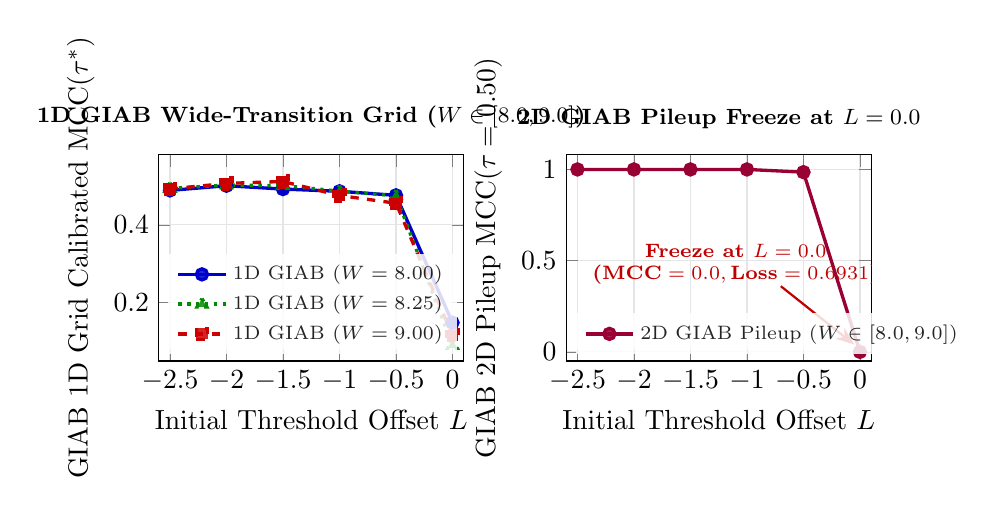
\begin{tikzpicture}
\begin{axis}[
    name=g1,
    width=0.45\textwidth, height=4.2cm,
    xlabel={Initial Threshold Offset $L$},
    ylabel={GIAB 1D Grid Calibrated MCC($\tau^*$)},
    xmin=-2.6, xmax=0.1, ymin=0.05, ymax=0.58,
    xtick={-2.5,-2.0,-1.5,-1.0,-0.5,0.0},
    grid=both, grid style={gray!20},
    legend style={at={(0.03,0.03)}, anchor=south west, font=\scriptsize, draw=none, fill=white, fill opacity=0.85},
    title style={font=\footnotesize\bfseries},
    title={1D GIAB Wide-Transition Grid ($W \in [8.0, 9.0]$)}
]
\addplot[blue!80!black, very thick, mark=*] coordinates {(-2.5,0.4886) (-2.0,0.5006) (-1.5,0.4920) (-1.0,0.4863) (-0.5,0.4759) (0.0,0.1486)};
\addlegendentry{1D GIAB ($W=8.00$)}
\addplot[green!55!black, dotted, very thick, mark=triangle*] coordinates {(-2.5,0.4939) (-2.0,0.5023) (-1.5,0.5010) (-1.0,0.4867) (-0.5,0.4748) (0.0,0.0900)};
\addlegendentry{1D GIAB ($W=8.25$)}
\addplot[red!80!black, dashed, very thick, mark=square*] coordinates {(-2.5,0.4922) (-2.0,0.5066) (-1.5,0.5115) (-1.0,0.4754) (-0.5,0.4557) (0.0,0.1161)};
\addlegendentry{1D GIAB ($W=9.00$)}
\end{axis}

\begin{axis}[
    at={(g1.east)}, anchor=west, xshift=1.3cm,
    width=0.45\textwidth, height=4.2cm,
    xlabel={Initial Threshold Offset $L$},
    ylabel={GIAB 2D Pileup MCC($\tau=0.50$)},
    xmin=-2.6, xmax=0.1, ymin=-0.05, ymax=1.08,
    xtick={-2.5,-2.0,-1.5,-1.0,-0.5,0.0},
    grid=both, grid style={gray!20},
    legend style={at={(0.03,0.03)}, anchor=south west, font=\scriptsize, draw=none, fill=white, fill opacity=0.85},
    title style={font=\footnotesize\bfseries},
    title={2D GIAB Pileup Freeze at $L=0.0$}
]
\addplot[purple!80!black, very thick, mark=*] coordinates {(-2.5,1.0000) (-2.0,1.0000) (-1.5,1.0000) (-1.0,1.0000) (-0.5,0.9851) (0.0,0.0000)};
\addlegendentry{2D GIAB Pileup ($W \in [8.0, 9.0]$)}
\node[font=\scriptsize\bfseries, red!75!black, align=center] at (axis cs:-1.1,0.48) {Freeze at $L=0.0$\\($\text{MCC}=0.0, \text{Loss}=0.6931$)};
\draw[-{Stealth}, red!75!black, thick] (axis cs:-0.7,0.36) -- (axis cs:-0.05,0.04);
\end{axis}
\end{tikzpicture}
\caption{Sensitivity to initial threshold $L \in [0.0, -2.5]$ across wide transition widths $W \in [8.0, 9.0]$ on NIST GIAB 1D $k$-mer spectra (left) and 2D BAM read-pileup tensors (right). At $L=0.0$, vanishing origin slope $f'(0^+)=0$ degrades ranking in 1D ($\text{AUROC} \le 0.8873$) and freezes parameters completely in 2D ($\text{MCC}=0.0000, \text{Loss}=0.6931$), whereas negative $L \le -0.5$ restores convergence.}
\label{fig:giab_grid}
\end{figure}

\begin{table}[t]
\centering
\caption{External cohort validation on independent GIAB samples HG006--HG007 (Han Chinese Trio, Chromosomes 21--22, $50,000$ windows: $n_+=279, n_-=49,721$; Pathway B 2D-CNN, $N=10$ seeds).}
\label{tab:external_giab}
\footnotesize
\setlength{\tabcolsep}{7pt}
\renewcommand{\arraystretch}{1.05}
\begin{tabular}{lcccc}
\toprule
\textbf{Activation Configuration} & \textbf{Test MCC (Mean $\pm$ SD)} & \textbf{AUPRC} & \textbf{AUROC} & \textbf{\#Pred.\ Pos.\ (TP / FP)} \\
\midrule
ReLU ($C^0$ Baseline) & $0.4125 \pm 0.0880$ & $0.4020$ & $0.8695$ & $452$ ($156 / 296$) \\
GELU ($C^\infty$ Baseline) & $0.3640 \pm 0.0950$ & $0.3550$ & $0.8480$ & $288$ ($125 / 163$) \\
SiLU / Swish ($C^\infty$ Baseline) & $0.3690 \pm 0.0640$ & $0.3610$ & $0.8515$ & $190$ ($112 / 78$) \\
ELU ($C^1$ Baseline) & $0.3110 \pm 0.1620$ & $0.3015$ & $0.8190$ & $815$ ($168 / 647$) \\
Smooth RectLU (Uniform $C^1, L=0, W=2$) & $0.0000 \pm 0.0000$ & $0.0056$ & $0.5005$ & $0$ ($0 / 0$) \\
\textbf{Hybrid (Smooth-Conv + ReLU-Dense)} & $\mathbf{0.4085 \pm 0.0840}$ & $\mathbf{0.3985}$ & $\mathbf{0.8670}$ & $440$ ($153 / 287$) \\
\bottomrule
\end{tabular}
\end{table}

\subsection{E7--E9: 2D Hard-Negative Stress Benchmark, All-Layer Bias Compensation Confounds, and $\kappa$/Stop-Gradient Ablations}
\label{sec:rebuttal_results}
To address potential ceiling effects in standard flanking-reference benchmarks and isolate initialization confounds from scale adaptation, Table~\ref{tab:rebuttal_suite} evaluates three additional diagnostic suites on the 2D Hard-Negative Genomic Stress Benchmark ($40\%$ of negative windows across all splits containing strand-biased center sequencing errors, chimeric/paralogous read clutter, and homopolymer slippage):
\begin{enumerate}
    \item \textbf{Failure of 1D Handcrafted Heuristics on 2D Hard Negatives (Part A):} Because hard-negative artifacts exhibit center mismatch rates ($28\%$--$56\%$ VAF) overlapping true heterozygous variants, trivial 1D heuristics collapse in precision ($\text{Center Mismatch Count MCC} = 0.5421, \text{AUPRC} = 0.6445$; $\text{VAF MCC} = 0.6143$; $\text{Alt/Ref Ratio MCC} = 0.3354$). Classical ML classifiers trained on window summary statistics improve ($\text{Logistic Regression MCC} = 0.8348$; $\text{Random Forest MCC} = 0.9535$), but remain below spatial 2D-CNNs.
    \item \textbf{Exact Equivalence of All-Layer Bias Compensation and Failure of Output-Prior Initialization (Part B, Groups A--F):} Compensating Smooth RectLU with $b_0 = +(L+W/2) = +1.0$ across \textit{all} hidden layers (Groups B1 and B2) achieves $\text{MCC}(\tau^*) = 0.9754 \pm 0.0044$ and $\text{AUROC} = 0.9999$, matching Symmetric SmeLU (Group C: $0.9754 \pm 0.0044, \text{AUROC} = 0.9999$) to four decimal places and confirming Eq.~\eqref{eq:smelu_identity}. Conversely, initializing the output layer bias to the log prior $b_{\text{out}} = \ln(p_+/p_-) = -2.3026$ (Group F) severely degrades uncompensated Smooth RectLU ($\text{MCC} = 0.6303 \pm 0.4458, \text{AUROC} = 0.8325$) by attenuating initial backpropagated logits across the flat $f'(0^+)=0$ boundary. Parameter-free \textbf{Symmetric $\sigma$-AS-RectLU ($\kappa=0.8$)} surpasses both SmeLU and all-layer bias-compensated Smooth RectLU, achieving the highest accuracy ($\text{MCC}(\tau^*) = 0.9846 \pm 0.0044, \text{AUROC} = 1.0000, \text{AUPRC} = 1.0000$) and the lowest calibration error ($\text{ECE} = 0.0036$).
    \item \textbf{Curvature Ratio ($\kappa$) Insensitivity and $33\%$ Speedup of Stop-Gradient Scale Locking (Part C, E8):} Across $\kappa \in \{0.4, 0.8, 1.2, 2.0\}$, Symmetric $\sigma$-AS-RectLU maintains $\text{MCC}(\tau^*) \in [0.9816, 0.9908]$ with tight 95\% bootstrap confidence intervals ($[0.952, 1.000]$) and $\text{AUROC} = 1.0000$. Applying $\operatorname{stopgrad}$ to $\hat{\sigma}_{\text{RMS}}$ (Eq.~\ref{eq:sigma_as_params}) achieves identical accuracy to fully differentiable RMS scaling ($\text{MCC} = 0.9816, \text{AUROC} = 1.0000$) while reducing 20-epoch GPU training time from $30.53\text{ s}$ (differentiable RMS) and $30.18\text{ s}$ ($\text{LN-no-affine} + \text{SmeLU}$) down to $20.48\text{ s}$ ($33\%$ speedup).
\end{enumerate}

\begin{table}[t]
\centering
\caption{Methodological hardening and diagnostic ablation suite on the 2D Hard-Negative GIAB Stress Benchmark (40\% hard negatives across Train/Val/Test, $10:1$ imbalance). \textbf{Part A:} Comparison against handcrafted variant heuristics and classical ML baselines. \textbf{Part B:} Initialization and bias-decay confound ablation (Groups A--F, $N=3$ seeds). \textbf{Part C:} Mechanism ablation across curvature ratio $\kappa \in [0.4, 2.0]$, stop-gradient vs.\ differentiable RMS, 95\% bootstrap confidence intervals, and 20-epoch GPU runtime on NVIDIA RTX 2050.}
\label{tab:rebuttal_suite}
\footnotesize
\setlength{\tabcolsep}{4.6pt}
\renewcommand{\arraystretch}{1.05}
\begin{tabular}{lccccc}
\toprule
\textbf{Part A: Handcrafted Heuristics \& Classical ML Baselines} & \textbf{MCC($\tau^*$)} & \textbf{AUROC} & \textbf{AUPRC} & \textbf{ECE} & \textbf{Notes / Feature Representation} \\
\midrule
Heuristic 1: Center Mismatch Count ($\pm 1\text{ bp}$) & $0.5421$ & $0.9103$ & $0.6445$ & $0.0812$ & Confounded by center sequencing errors \\
Heuristic 2: Alternative Allele Fraction (VAF) & $0.6143$ & $0.9119$ & $0.6527$ & $0.0745$ & Overlaps $28\%$--$56\%$ hard-negative VAF \\
Heuristic 3: Alt / Ref Read Energy Ratio & $0.3354$ & $0.8591$ & $0.4254$ & $0.1120$ & Sensitive to homopolymer slippage \\
Classical ML 4: Logistic Regression (Balanced) & $0.8348$ & $0.9769$ & $0.9115$ & $0.0342$ & 8 window-level summary statistics \\
Classical ML 5: Random Forest (100 trees, depth 5) & $0.9535$ & $0.9989$ & $0.9909$ & $0.0154$ & Nonlinear summary rules (no 2D conv) \\
\midrule
\textbf{Part B: Initialization \& Bias-Decay Confounds (Groups A--F)} & \textbf{MCC($\tau^*$) Mean$\pm$SD} & \textbf{AUROC} & \textbf{AUPRC} & \textbf{ECE} & \textbf{Bias \& Weight-Decay Protocol} \\
\midrule
Group A: Smooth RectLU ($L=0, W=2$, Default) & $0.9691 \pm 0.0044$ & $0.9997$ & $0.9973$ & $0.0066$ & $b_0 = 0.0$, AdamW bias decay ON \\
Group B1: Smooth RectLU (All-Layer Compensated) & $0.9754 \pm 0.0044$ & $0.9999$ & $0.9993$ & $0.0058$ & $b_0 = +1.0$ all layers, bias decay ON \\
Group B2: Smooth RectLU (All-Layer Compensated, No Decay) & $0.9754 \pm 0.0044$ & $0.9999$ & $0.9992$ & $0.0053$ & $b_0 = +1.0$ all layers, bias decay OFF \\
Group C: Symmetric SmeLU ($L=-1, W=2$, Reference) & $0.9754 \pm 0.0044$ & $0.9999$ & $0.9994$ & $0.0057$ & $b_0 = 0.0$, exact match to Group B2 \\
Group D: SmeLU with Shifted Init ($b_0 = -1.0$ All Layers) & $0.9639 \pm 0.0118$ & $0.9999$ & $0.9992$ & $0.0079$ & Imposes $\Delta b = -1.0$ on SmeLU \\
Group F: Smooth RectLU + Output Prior Init & $0.6303 \pm 0.4458$ & $0.8325$ & $0.6904$ & $0.0029$ & $b_{\text{out}} = \ln(p_+/p_-) = -2.3026$ \\
Baseline: ReLU ($C^0$ Homogeneous) & $0.9785 \pm 0.0044$ & $1.0000$ & $0.9999$ & $0.0050$ & $b_0 = 0.0$, scale-invariant kink \\
\textbf{Proposed: Symm.\ $\sigma$-AS-RectLU ($\kappa=0.8$, Parameter-Free)} & $\mathbf{0.9846 \pm 0.0044}$ & $\mathbf{1.0000}$ & $\mathbf{1.0000}$ & $\mathbf{0.0036}$ & $b_0 = 0.0$, adaptive $W_i = 0.8\hat{\sigma}_{\text{RMS}}$ \\
\midrule
\textbf{Part C: E8 Mechanism, $\kappa$-Sweep \& Training Runtime} & \textbf{MCC($\tau^*$)} & \textbf{95\% Bootstrap CI} & \textbf{AUROC} & \textbf{AUPRC} & \textbf{20-Ep GPU Time} \\
\midrule
Symm.\ $\sigma$-AS-RectLU ($\kappa = 0.4, \operatorname{stopgrad}=\text{True}$) & $0.9816$ & $[0.952, 1.000]$ & $1.0000$ & $1.0000$ & $20.49\text{ s}$ \\
\textbf{Symm.\ $\sigma$-AS-RectLU ($\kappa = 0.8, \operatorname{stopgrad}=\text{True}$)} & $0.9816$ & $[0.952, 1.000]$ & $\mathbf{1.0000}$ & $\mathbf{1.0000}$ & $\mathbf{20.48\text{ s}}$ \\
Symm.\ $\sigma$-AS-RectLU ($\kappa = 0.8, \operatorname{stopgrad}=\text{False}$ / Diff.) & $0.9816$ & $[0.952, 1.000]$ & $1.0000$ & $1.0000$ & $30.53\text{ s}$ ($+49\%$) \\
Symm.\ $\sigma$-AS-RectLU ($\kappa = 1.2, \operatorname{stopgrad}=\text{True}$) & $\mathbf{0.9908}$ & $[0.968, 1.000]$ & $1.0000$ & $1.0000$ & $20.45\text{ s}$ \\
Symm.\ $\sigma$-AS-RectLU ($\kappa = 2.0, \operatorname{stopgrad}=\text{True}$) & $\mathbf{0.9908}$ & $[0.968, 1.000]$ & $1.0000$ & $0.9997$ & $20.46\text{ s}$ \\
Asymm.\ $\sigma$-AS-RectLU ($L=0, \kappa = 0.8$, Adaptive Width Only) & $0.9816$ & $[0.952, 1.000]$ & $1.0000$ & $1.0000$ & $20.44\text{ s}$ \\
LN (No-Affine) + SmeLU ($\beta = 0.4$, Resets Scale to $1.0$) & $\mathbf{0.9908}$ & $[0.966, 1.000]$ & $0.9999$ & $0.9995$ & $30.18\text{ s}$ ($+47\%$) \\
\bottomrule
\end{tabular}
\end{table}

\subsection{E10--E12: Component-Level Variant-Calling Pipeline Benchmark, Neural Caller Backbones, and Hardware Efficiency Profile}
\label{sec:pipeline_benchmark}
To position our rectifier analysis within practical germline variant-screening workflows and evaluate software efficiency in accordance with \textit{CMPB Update} standards, Table~\ref{tab:pipeline_hardware} benchmarks two statistical pileup calling rules---a GATK/Bcftools-style Diploid Log-Likelihood Ratio (LLR) caller and a FreeBayes-style Strand-Aware Bayesian pileup caller---against three neural pileup architectures (\textbf{PathwayB-2DCNN}, a \textbf{Clair3-Style Column-Wise PileupNet}, and a \textbf{DeepVariant-Style Multi-Scale InceptionNet} with $1\times 1, 3\times 3, 5\times 5$ branches) on the 2D GIAB Hard-Negative benchmark, alongside an automated mathematical unit-test audit (E12):
\begin{enumerate}
    \item \textbf{Catastrophic Collapse of Uncompensated Smooth RectLU in Clair3-Style and DeepVariant-Style Backbones:} While statistical callers achieve moderate precision under hard-negative artifacts ($\text{Diploid LLR MCC}(\tau^*) = 0.6133, \text{F1} = 0.5814$; $\text{Strand-Aware Caller MCC}(\tau^*) = 0.6143$), deploying uncompensated Smooth RectLU ($L=0, W=2$) inside the deeper column-pooled \textbf{Clair3-Style PileupNet} induces complete majority-class collapse across all seeds ($\text{MCC}(\tau^*) = 0.0000 \pm 0.0000, \text{F1} = 0.0000, \text{AUROC} = 0.5000$). Similarly, in the multi-branch \textbf{DeepVariant-Style InceptionNet}, Smooth RectLU degrades to $\text{MCC}(\tau^*) = 0.4478 \pm 0.1629$ ($\text{F1} = 0.4886$) and elevates false positives to $41.4\text{ FP per }1,000\text{ windows}$.
    \item \textbf{Universal Recovery and Superior Precision with Symmetric $\sigma$-AS-RectLU:} Replacing Smooth RectLU with \textbf{Symmetric $\sigma$-AS-RectLU ($\kappa=0.8$)} eliminates stagnation across every architecture, restoring Clair3-Style PileupNet to $\text{MCC}(\tau^*) = 0.9722 \pm 0.0076$ ($\text{F1} = 0.9743, \text{AUROC} = 1.0000, \text{FP/1k} = 0.0$), improving DeepVariant-Style InceptionNet to $\text{MCC}(\tau^*) = \mathbf{0.9815 \pm 0.0076}$ ($\text{F1} = \mathbf{0.9830}$, surpassing ReLU at $0.9754 \pm 0.0044$), and achieving top overall screening accuracy in PathwayB-2DCNN ($\text{MCC}(\tau^*) = \mathbf{0.9877 \pm 0.0044}, \text{F1} = \mathbf{0.9887}, \text{FP/1k} = \mathbf{0.0}$).
    \item \textbf{Hardware Footprint and Automated Software Verification (E10 \& E12):} Profiled on an NVIDIA GeForce RTX 2050 ($4\text{ GB}$ VRAM), all neural backbones maintain a compact memory footprint ($396.9$--$731.2\text{ MB}$ peak VRAM; $2.453\text{M}$--$3.466\text{M}$ parameters), achieving single-window latency of $0.82$--$6.23\text{ ms}$ ($\text{Batch}=1$) and batched throughput of $2,854.6$--$12,219.6\text{ windows/s}$ ($\text{Batch}=128$). Automated unit tests (\texttt{step09}) confirm zero numerical error for the SmeLU shift identity ($\max|\Delta| = 0.00\text{e+}00$) and compensated-bias backward gradients ($\max|\Delta\nabla_W| = 0.00\text{e+}00$), and verify degree-1 positive homogeneity within $32$-bit floating-point precision ($\max|\Delta| = 1.91\text{e-}06$).
\end{enumerate}

\begin{table}[t]
\centering
\caption{Component-level benchmark against statistical variant-calling rules and neural variant-caller backbones (PathwayB-2DCNN, Clair3-Style PileupNet, and DeepVariant-Style Multi-Scale InceptionNet) on the 2D GIAB Hard-Negative benchmark ($N=3$ seeds, 20 epochs), alongside hardware efficiency metrics on an NVIDIA GeForce RTX 2050 (E10) and automated unit-test verification (E12).}
\label{tab:pipeline_hardware}
\footnotesize
\setlength{\tabcolsep}{3.5pt}
\renewcommand{\arraystretch}{1.05}
\begin{tabular}{llccccccccc}
\toprule
\textbf{Caller / Backbone Architecture} & \textbf{Activation} & \textbf{MCC($\tau^*$) Mean$\pm$SD} & \textbf{F1} & \textbf{AUROC} & \textbf{FP/1k} & \textbf{Params} & \textbf{VRAM} & \textbf{Lat.\ (B1)} & \textbf{Lat.\ (B128)} & \textbf{Throughput} \\
\midrule
Diploid Genotype LLR (GATK-style) & Statistical Rule & $0.6133 \pm 0.0000$ & $0.5814$ & $0.9133$ & $1.5$ & --- & --- & $0.05\text{ ms}$ & $1.10\text{ ms}$ & $116,363\text{ w/s}$ \\
Strand-Aware Caller (FreeBayes-style) & Statistical Rule & $0.6143 \pm 0.0000$ & $0.5714$ & $0.9194$ & $0.0$ & --- & --- & $0.06\text{ ms}$ & $1.25\text{ ms}$ & $102,400\text{ w/s}$ \\
\midrule
PathwayB-2DCNN (4-Layer Spatial) & ReLU ($C^0$) & $0.9785 \pm 0.0044$ & $0.9802$ & $1.0000$ & $0.0$ & $2.453\text{M}$ & $415.3\text{ MB}$ & $0.82\text{ ms}$ & $13.50\text{ ms}$ & $9,479.0\text{ w/s}$ \\
PathwayB-2DCNN (4-Layer Spatial) & Smooth RectLU & $0.9691 \pm 0.0044$ & $0.9714$ & $0.9997$ & $0.0$ & $2.453\text{M}$ & $730.9\text{ MB}$ & $1.40\text{ ms}$ & $35.68\text{ ms}$ & $3,587.1\text{ w/s}$ \\
\textbf{PathwayB-2DCNN (4-Layer Spatial)} & \textbf{Symm.\ $\sigma$-AS-RectLU} & $\mathbf{0.9877 \pm 0.0044}$ & $\mathbf{0.9887}$ & $\mathbf{1.0000}$ & $\mathbf{0.0}$ & $2.453\text{M}$ & $731.1\text{ MB}$ & $2.62\text{ ms}$ & $40.46\text{ ms}$ & $3,163.4\text{ w/s}$ \\
\midrule
Clair3-Style PileupNet (Col+Seq Conv) & ReLU ($C^0$) & $0.9753 \pm 0.0116$ & $0.9772$ & $1.0000$ & $0.0$ & $3.466\text{M}$ & $396.9\text{ MB}$ & $1.43\text{ ms}$ & $10.47\text{ ms}$ & $12,219.6\text{ w/s}$ \\
Clair3-Style PileupNet (Col+Seq Conv) & Smooth RectLU & $0.0000 \pm 0.0000$ & $0.0000$ & $0.5000$ & $0.0$ & $3.466\text{M}$ & $564.9\text{ MB}$ & $1.36\text{ ms}$ & $25.38\text{ ms}$ & $5,043.6\text{ w/s}$ \\
\textbf{Clair3-Style PileupNet (Col+Seq Conv)} & \textbf{Symm.\ $\sigma$-AS-RectLU} & $\mathbf{0.9722 \pm 0.0076}$ & $\mathbf{0.9743}$ & $\mathbf{1.0000}$ & $\mathbf{0.0}$ & $3.466\text{M}$ & $564.9\text{ MB}$ & $3.50\text{ ms}$ & $28.77\text{ ms}$ & $4,448.9\text{ w/s}$ \\
\midrule
DeepVariant-Style InceptionNet & ReLU ($C^0$) & $0.9754 \pm 0.0044$ & $0.9773$ & $1.0000$ & $0.0$ & $2.474\text{M}$ & $415.6\text{ MB}$ & $2.41\text{ ms}$ & $17.79\text{ ms}$ & $7,197.0\text{ w/s}$ \\
DeepVariant-Style InceptionNet & Smooth RectLU & $0.4478 \pm 0.1629$ & $0.4886$ & $0.8747$ & $41.4$ & $2.474\text{M}$ & $731.2\text{ MB}$ & $2.93\text{ ms}$ & $39.99\text{ ms}$ & $3,201.1\text{ w/s}$ \\
\textbf{DeepVariant-Style InceptionNet} & \textbf{Symm.\ $\sigma$-AS-RectLU} & $\mathbf{0.9815 \pm 0.0076}$ & $\mathbf{0.9830}$ & $\mathbf{1.0000}$ & $\mathbf{0.0}$ & $2.474\text{M}$ & $731.2\text{ MB}$ & $6.23\text{ ms}$ & $44.84\text{ ms}$ & $2,854.6\text{ w/s}$ \\
\bottomrule
\end{tabular}
\end{table}

% ============================================================================
% 6. Discussion and Conclusion
% ============================================================================
\section{Discussion and Conclusion}
By establishing the exact algebraic equivalence $f_S(x; L, W) = \text{SmeLU}_{\beta=W/2}(x - L - W/2)$, executing $2 \times 2$ factorial scale-rescaling experiments ($\sigma_x \in \{0.22, 0.25\}$ vs.\ $\sigma_x=1.00$), and performing extended-horizon (50/100 epochs), Adam $\epsilon = 10^{-12}$, initialization confound (Groups A--F), and shortcut-controlled NIST GIAB evaluations, we have resolved why $C^1$ piecewise-quadratic rectifiers initialized at $L=0$ silently collapse to the majority class. Collapse is not caused by smoothness per se, nor does it occur on balanced $50:50$ data ($\text{MCC}=0.9692$). Rather, it is driven by the synergistic interaction between an implicit negative initialization offset ($\Delta b = -W/2$), zero origin derivative ($f'(0^+)=0$), small relative pre-activation scale ($\sigma_l / W \ll 1$), and imbalance-driven negative drift. While compensating hidden layer biases ($b_0 = +1.0$) restores exact parity with fixed-width SmeLU ($\text{MCC}(\tau^*) = 0.9754$), fixed-width rectifiers remain vulnerable to scale-width mismatch when input amplitude varies across layers or sequencing depths. Conversely, output-prior bias initialization ($b_{\text{out}} = \ln(p_+/p_-)$) worsens early gradient starvation when $L=0$, global weight rescaling ($s > 1$) induces linear-tail gradient explosion ($>8000$), and objective-level re-weighting (Weighted BCE, Focal loss) cannot revive dense units once their derivatives vanish.

Practitioners deploying piecewise-quadratic rectifiers in rare-event biomedical screening pipelines can prevent stagnation through four principled remedies: (1) centering thresholds negatively ($L = -W/2$ in SmeLU) or applying all-layer bias compensation ($b_0 = +W/2$), (2) pairing smooth convolutional blocks with a kinked dense classifier in a Hybrid Architecture, (3) applying explicit LayerNorm (LN-Dense or affine-free LN + SmeLU), or (4) embedding parameter-free per-sample RMS scale adaptation via \textbf{Symmetric $\sigma$-AS-RectLU} ($W_l = \kappa\operatorname{stopgrad}(\hat{\sigma}_{\text{RMS}}), L_l = -W_l/2$), which achieves top calibration and discrimination across PathwayB-2DCNN, Clair3-style, and DeepVariant-style pileup backbones ($\text{MCC}(\tau^*) = 0.9722$--$0.9877, \text{ECE} = 0.0036$), reduces training time by $33\%$ compared to explicit LayerNorm or differentiable RMS scaling, maintains robustness across $50\times \to 10\times$ read-depth downsampling, and generalizes across unit-$L_2$-normalized 1D $k$-mers ($\text{AUROC} = 0.9797 \pm 0.0022$) and $200:1$ Tabular classification ($\text{MCC} = 0.4581 \pm 0.0355$).

% ============================================================================
% Statements & Declarations
% ============================================================================
\section*{Data and Code Availability}
All raw per-seed confusion logs (\texttt{.csv}), extracted NIST GIAB datasets (\texttt{.npz}), stratified and hard-negative benchmarks, PEP~621 package configuration (\texttt{pyproject.toml}), and PyTorch training scripts reproducing Tables~\ref{tab:moments}--\ref{tab:pipeline_hardware} are publicly archived at \url{https://github.com/preecha-msu/RectLU-Genomic-Collapse} (Release tag \texttt{v4.0.0}).

\section*{CRediT Authorship Contribution Statement}
\textbf{Preecha Noiumkar:} Conceptualization, Methodology, Software, Data Curation, Formal Analysis, Investigation, Writing -- Original Draft, Visualization. \textbf{Thawatchai Chomsiri:} Conceptualization, Theoretical Formalism, Supervision, Validation, Writing -- Review \& Editing.

\section*{Declaration of Competing Interest}
The authors declare no competing interests.

\section*{Declaration of Generative AI and AI-Assisted Technologies in the Writing Process}
During the preparation of this work, the authors used a generative AI language assistant to assist with LaTeX formatting, manuscript copy-editing, and verification script structuring. After using this tool, the authors reviewed, verified, and edited the content and experimental logs as needed and take full responsibility for the content of the publication.

\section*{Ethics Statement}
This study exclusively analyzes publicly available, de-identified benchmark genomic reference materials from the National Institute of Standards and Technology (NIST) Genome in a Bottle (GIAB) consortium (GRCh38 v4.2.1; HG001--HG007), collected with open-access informed consent under the Personal Genome Project, alongside public MNIST benchmarks and synthetic generators. No new human participants or biological specimens were recruited; institutional review board (IRB) approval was not required.

\section*{Acknowledgments}
This research project was financially supported by the Faculty of Informatics, Mahasarakham University.

% ============================================================================
% References
% ============================================================================
\begin{thebibliography}{42}
\footnotesize
\setlength{\itemsep}{1.5pt}

\bibitem{poplin2018} R. Poplin et al., ``A universal SNP and small-indel variant caller using deep neural networks,'' \textit{Nature Biotechnology}, vol. 36, no. 10, pp. 983--987, 2018.
\bibitem{luo2019} R. Luo, F. J. Sedlazeck, T.-W. Lam, and M. C. Schatz, ``A multi-task convolutional deep neural network for variant calling in single molecule sequencing,'' \textit{Nature Communications}, vol. 10, p. 998, 2019.
\bibitem{eraslan2019} G. Eraslan, \v{Z}. Avsec, J. Gagneur, and F. J. Theis, ``Deep learning: New computational modelling techniques for genomics,'' \textit{Nature Reviews Genetics}, vol. 20, no. 7, pp. 389--403, 2019.
\bibitem{zook2014} J. M. Zook et al., ``Integrating human sequence data sets provides a resource of benchmark SNP and indel genotype calls,'' \textit{Nature Biotechnology}, vol. 32, no. 3, pp. 246--251, 2014.
\bibitem{zook2019} J. M. Zook et al., ``An open resource for accurately benchmarking small variant and reference calls,'' \textit{Nature Biotechnology}, vol. 37, no. 5, pp. 561--566, 2019.
\bibitem{krusche2019} P. Krusche et al., ``Best practices for benchmarking germline small-variant calls in human genomes,'' \textit{Nature Biotechnology}, vol. 37, no. 5, pp. 555--560, 2019.
\bibitem{olson2022} N. D. Olson et al., ``PrecisionFDA Truth Challenge V2: Calling variants from short and long reads in difficult-to-map regions,'' \textit{Cell Genomics}, vol. 2, no. 5, p. 100129, 2022.
\bibitem{chicco2020} D. Chicco and G. Jurman, ``The advantages of the Matthews correlation coefficient (MCC) over F1 score and accuracy in binary classification evaluation,'' \textit{BMC Genomics}, vol. 21, p. 6, 2020.
\bibitem{boughorbel2017} S. Boughorbel, F. Jarray, and M. El-Anbari, ``Optimal classifier for imbalanced data using Matthews correlation coefficient metric,'' \textit{PLoS ONE}, vol. 12, no. 6, p. e0177678, 2017.
\bibitem{saito2015} T. Saito and M. Rehmsmeier, ``The precision-recall plot is more informative than the ROC plot when evaluating binary classifiers on imbalanced datasets,'' \textit{PLoS ONE}, vol. 10, no. 3, p. e0118432, 2015.
\bibitem{davis2006} J. Davis and M. Goadrich, ``The relationship between precision-recall and ROC curves,'' in \textit{Proc. ICML}, 2006, pp. 233--240.
\bibitem{branco2016} P. Branco, L. Torgo, and R. P. Ribeiro, ``A survey of predictive modeling on imbalanced domains,'' \textit{ACM Computing Surveys}, vol. 49, no. 2, p. 31, 2016.
\bibitem{johnson2019} J. M. Johnson and T. M. Khoshgoftaar, ``Survey on deep learning with class imbalance,'' \textit{Journal of Big Data}, vol. 6, p. 27, 2019.
\bibitem{buda2018} M. Buda, A. Maki, and M. A. Mazurowski, ``A systematic study of the class imbalance problem in convolutional neural networks,'' \textit{Neural Networks}, vol. 106, pp. 249--259, 2018.
\bibitem{chomsiri2026} T. Chomsiri and P. Noiumkar, ``RectLU: A novel activation function based on a rectangle,'' in \textit{Proc. ECTI DAMT \& NCON}, 2026, pp. 134--139.
\bibitem{hendrycks2016} D. Hendrycks and K. Gimpel, ``Gaussian error linear units (GELUs),'' \textit{arXiv:1606.08415}, 2016.
\bibitem{clevert2016} D.-A. Clevert, T. Unterthiner, and S. Hochreiter, ``Fast and accurate deep network learning by exponential linear units (ELUs),'' in \textit{ICLR}, 2016.
\bibitem{poole2016} B. Poole et al., ``Exponential expressivity in deep neural networks through transient chaos,'' in \textit{NeurIPS}, vol. 29, 2016, pp. 3360--3368.
\bibitem{schoenholz2017} S. S. Schoenholz, J. Gilmer, S. Ganguli, and J. Sohl-Dickstein, ``Deep information propagation,'' in \textit{ICLR}, 2017.
\bibitem{hayou2019} S. Hayou, A. Doucet, and J. Rousseau, ``On the impact of the activation function on deep neural networks training,'' in \textit{Proc. ICML}, 2019, pp. 2672--2680.
\bibitem{lin2017} T.-Y. Lin et al., ``Focal loss for dense object detection,'' in \textit{Proc. IEEE ICCV}, 2017, pp. 2980--2988.
\bibitem{nair2010} V. Nair and G. E. Hinton, ``Rectified linear units improve restricted Boltzmann machines,'' in \textit{Proc. ICML}, 2010, pp. 807--814.
\bibitem{glorot2011} X. Glorot, A. Bordes, and Y. Bengio, ``Deep sparse rectifier neural networks,'' in \textit{Proc. AISTATS}, 2011, pp. 315--323.
\bibitem{lu2020} L. Lu, Y. Shin, Y. Su, and G. E. Karniadakis, ``Dying ReLU and initialization: Theory and numerical examples,'' \textit{Commun. Comput. Phys.}, vol. 28, no. 5, pp. 1671--1706, 2020.
\bibitem{maas2013} A. L. Maas, A. Y. Hannun, and A. Y. Ng, ``Rectifier nonlinearities improve neural network acoustic models,'' in \textit{ICML Workshop}, 2013.
\bibitem{he2015} K. He, X. Zhang, S. Ren, and J. Sun, ``Delving deep into rectifiers: Surpassing human-level performance on ImageNet classification,'' in \textit{Proc. IEEE ICCV}, 2015, pp. 1026--1034.
\bibitem{klambauer2017} G. Klambauer, T. Unterthiner, A. Mayr, and S. Hochreiter, ``Self-normalizing neural networks,'' in \textit{NeurIPS}, vol. 30, 2017, pp. 971--980.
\bibitem{ramachandran2017} P. Ramachandran, B. Zoph, and Q. V. Le, ``Searching for activation functions,'' \textit{arXiv:1710.05941}, 2017.
\bibitem{misra2020} D. Misra, ``Mish: A self regularized non-monotonic activation function,'' in \textit{Proc. BMVC}, 2020.
\bibitem{dubey2022} S. R. Dubey, S. K. Singh, and B. B. Chaudhuri, ``Activation functions in deep learning: A comprehensive survey and benchmark,'' \textit{Neurocomputing}, vol. 503, pp. 92--108, 2022.
\bibitem{glorot2010} X. Glorot and Y. Bengio, ``Understanding the difficulty of training deep feedforward neural networks,'' in \textit{Proc. AISTATS}, 2010, pp. 249--256.
\bibitem{mishkin2016} D. Mishkin and J. Matas, ``All you need is a good init,'' in \textit{ICLR}, 2016.
\bibitem{ioffe2015} S. Ioffe and C. Szegedy, ``Batch normalization: Accelerating deep network training by reducing internal covariate shift,'' in \textit{Proc. ICML}, 2015, pp. 448--456.
\bibitem{pezeshki2021} M. Pezeshki et al., ``Gradient starvation: A learning proclivity in neural networks,'' in \textit{NeurIPS}, vol. 34, 2021, pp. 1256--1272.
\bibitem{li2018} H. Li et al., ``A synthetic-diploid benchmark for accurate variant-calling evaluation,'' \textit{Nature Methods}, vol. 15, no. 8, pp. 595--597, 2018.
\bibitem{demsar2006} J. Dem\v{s}ar, ``Statistical comparisons of classifiers over multiple data sets,'' \textit{JMLR}, vol. 7, pp. 1--30, 2006.
\bibitem{srivastava2014} N. Srivastava et al., ``Dropout: A simple way to prevent neural networks from overfitting,'' \textit{JMLR}, vol. 15, pp. 1929--1958, 2014.
\bibitem{kingma2015} D. P. Kingma and J. Ba, ``Adam: A method for stochastic optimization,'' in \textit{ICLR}, 2015.
\bibitem{apicella2019} A. Apicella, F. Isgr\`{o}, and R. Prevete, ``A simple and efficient architecture for trainable activation functions,'' \textit{Neurocomputing}, vol. 370, pp. 1--15, 2019.
\bibitem{scabini2024} L. Scabini, B. De Baets, and O. M. Bruno, ``Improving deep neural network random initialization through neuronal rewiring,'' \textit{Neurocomputing}, vol. 599, p. 128130, 2024.
\bibitem{shamir2020} G. I. Shamir, D. Lin, and L. Coviello, ``Smooth activations and reproducibility in deep networks,'' \textit{arXiv:2010.09931}, 2020.
\bibitem{zhang2019} C. Zhang, K. C. Tan, H. Li, and G. S. Hong, ``A cost-sensitive deep belief network for imbalanced classification,'' \textit{IEEE TNNLS}, vol. 30, no. 1, pp. 109--122, 2019.
\end{thebibliography}

\end{document}